We have analysed more than 35000 time series of taxa from the gut microbiomes of 97 individuals (sampling from three up to 332 time points), obtained from publicly available high throughput sequencing data on: healthy individuals over a long term span\cite{moving}, people with various degrees of obesity\cite{LEA}, twin pairs discordant for kwashiorkor\cite{kwashiorkor}, response to diet changes\cite{diet} or to antibiotic perturbation\cite{antibiotic}, and subjects diagnosed with irritable bowel syndrome (IBS)\cite{IBS}. 
We engineered a complete software framework and a web platform, ComplexCruncher, ready to be implemented by other users.
  
We summarize our dataset in ST1-6 (Tables 1-6 in suplemental material). The bacteria and archaea taxonomic assignations were obtained by analysing 16S rRNA sequences, which were clustered into operational taxonomic units (OTUs) sharing 97 \% sequence identity using QIIME\cite{QIIME}. WGS data\cite{kwashiorkor} were analysed and assigned at strain level by the Livermore Metagenomic Analysis Toolkit (LMAT)\cite{LMAT}, according to their default quality threshold. Genus, with best balance between error assignment and number of taxa, was chosen as our reference taxonomic level. We have verified that our conclusions are not significantly affected by selecting family or species as the reference taxonomic level (see Figure 1 in supplemental material).

\todo{Specify, in each study treated, the nature of the samples (conditions, timespan between timepoints, subjects). Specify, and it is very important, what we consider ?healthy? in each study (for example: pre-antibiotics is healthy)}

%%%
\subsection*{Model} \label{sec:model}

We model the microbial abundances across time along the lines of Blumm \textit{et al.}\cite{ranking}. The dynamics of taxon relative abundances is described by the Langevin equation:
\begin{linenomath}
\begin{equation}
\dot{x_i} = F_i \cdot x_i^\alpha + V \cdot x_i^\beta \xi_i(t) - \phi(t) \cdot x_i,
\end{equation}
\end{linenomath}
where F$_i$ captures the fitness of the taxon i, V corresponds to the noise amplitude and $\xi_i$(t) is a Gaussian random noise with zero mean  $<\xi_i(t)>$ = 0 and variance uncorrelated in time, $<\xi_i(t) \xi_i(t')>$ =  $\delta(t'-t)$, . The function $\phi(t)$ ensures the normalization at all times, $\sum x_i(t) = 1$, and corresponds to $\phi(t) = \sum F_i x_i^\alpha + \sum V x_i^\beta \xi_i(t)$.
The temporal evolution of the probability that a taxon i has a relative abundance $x_i(t)$, P(x$_i$,t), is determined by the Fokker-Planck equation:
\begin{linenomath}
\begin{equation}
\frac{\partial P}{\partial t} = - \frac{\partial}{\partial x_i}  [(F_i \cdot x_i^\alpha - \phi(t) \cdot x_i ) \cdot P]+ \frac{1}{2} \frac{\partial^2}{\partial x_i^2} (V^2 \cdot x_i^{2\beta}\cdot P).
\end{equation}
\end{linenomath}
The microbiota evolves towards a steady-state with a time-independent probability depending on the values of $\alpha$, $\beta$, F$_i$ and V. For $\alpha<1$ (otherwise, systems are always unstable), the steady-state probability may be localized in a region around a preferred value or broadly distributed over a wide range, depending on whether the fitness F$_i$  dominates or is overwhelmed by the noise amplitude V. The steady-state solution of the Fokker-Planck equation is given by:
\begin{eqnarray}
P_0 (x_i) &=& C_{ne}(\alpha,\beta,F_i,V)  \cdot x_i^{-2\beta}  \cdot \exp\Big[\frac{2F_i}{V^2}\frac{x_i^{1+\alpha-2\beta}}{1+\alpha-2\beta}-\frac{\phi_0}{V^2}\frac{x_i^{2-2\beta}}{1-\beta}\Big] \quad \textrm{if} \quad  2\beta \ne 1+\alpha, \notag \\
P_0 (x_i) &=& C_e(\alpha,\beta,F_i,V)  \cdot x_i^{\frac{2F_i}{V^2} -2\beta}  \cdot \exp\Big[\frac{\phi_0}{V^2}\frac{x_i^{2-2\beta}}{1-\beta}\Big] \quad \textrm{if} \quad  2\beta = 1+\alpha,
\notag
\end{eqnarray}
where $\phi_0 = (\sum_i F_i^{1/(1-\alpha)})^{1-\alpha}$ and C$_{ne}$ and C$_{e}$ are integrals that should be solved numerically for the parameters of interest. The ordered phase happens when the solution has a maximum in the physical interval ($0<x_i<1$). For larger V, the transition to a disordered phase happens when the maximum shifts to the unphysical region $x_i<0$, which sets the phase transition region V($\alpha,\beta,F_i$). The phase transition region can be calculated analytically in particular cases:
\begin{eqnarray}
F_i^2 &=& 4 \beta \phi_0 V^2\quad \textrm{if} \quad  \beta = \alpha \neq 1, \notag \\
F_i &=& \beta V^2\quad \textrm{if} \quad  2\beta = 1+\alpha,
\notag
\end{eqnarray}
where the first case, simplifies to $F= 3 V^2$ if $\beta = 0.75$ and the fitness of this taxon dominates in $\phi_0$. 
In many physical systems (Brownian motion is the classical example), the two terms of the Langevin equation are related.  The \emph{fluctuation--dissipation theorem} states a general relationship between the response to an external disturbance and the internal fluctuations of the system\cite{FD}. The theorem can be used as the basic formula to derive the fitness from the analysis of fluctuations 
of the microbiota, assuming that it is in equilibrium (the ordered phase).  

\todo{Explain better the fluctiation-dissipation theorem}


%%%
\subsection*{Selection and Methods}

\subsubsection*{Sample selection}
We have chosen studies about relevant pathologies containing metagenomic sequencing time data series of bacterial populations from humans in different healthy and non-healthy states. We have selected only those individuals who had three or more time points of data available in databases. Metadata of each study is provided in Supplementary Tables \ref{tab:diet} to \ref{tab:LEA}. All used 16S rRNA gene sequencing except for the study of the discordant kwashiorkor twins\cite{kwashiorkor} (see Supplementary Tables \ref{tab:DH} and \ref{tab:DK}) where shotgun metagenomic sequencing (SMS) and 16S rRNA were used. In the latter case we selected to work with SMS data to show that our method is valid regardless of the source of taxonomic information. Each one of the datasets was treated as follows:

\subsubsection*{16rRNA sequences processing}
Reads from the selected studies were first quality filtered using the FastX toolkit\cite{FASTX}, allowing only those reads which had more than 25 of quality along the 75\% of the complete sequence. 16S rRNA reads were then clustered at 97\% nucleotide sequence identity (97\% ID) into operational taxonomic units (OTUs) using QIIME package software\cite{QIIME} (version 1.8) We followed open reference OTU picking workflow in all cases. The clustering method used was uclust, and the OTUs were matched against Silva database\cite{SILVA} (version 111, July 2012) and were assigned to taxonomy with an uclust-based consensus taxonomy assigner. The parameters used in this step were: similarity 0.97, prefilter percent id 0.6, max accepts 20, max rejects 500. 

\subsubsection*{Metagenomic sequences processing}
Metagenomic shotgun (and 16S too) sequences were analyzed with LMAT (Livermore Metagenomics Analysis Toolkit) software package\cite{LMAT} (version 1.2.4, with Feb'15 release of data base \emph{LMAT-Grand}). LMAT was run using a Bull shared-memory node belonging to the team's HPC (high performance computing) cluster. It is equipped with 32 cores (64 threads available using Intel Hyper-threading technology) as it has 2 Haswell-based Xeons, the E5-2698v3@2.3 GHz, sharing half a tebibyte (0.5 TiB, that is, 512 gibibytes) of DRAM memory. This node is also provided with a card PCIe SSD as NVRAM, the P420m HHHL, with 1.4 TB, and 750000 reading IOPS, 4 KB, achieving 3.3 GB/s, which Micron kindly issued free of charge, as a sample for testing purposes. The computing node was supplied with a RAID-0 (striping) scratch disk area. We used the ``Grand'' database\footnote{In this context, ``Grand'' refers to a huge database that contains k-mers from all viral, prokaryote, fungal and protist genomes present in the NCBI database, plus Human reference genome (hg19), plus GenBank Human, plus the 1000 Human Genomes Project (HGP). This represent about 31.75 billion k-mers occupying 457.62 GB.}, release Feb'15, provided by the LMAT team. Previously to any calculation, the full database was loaded in the NVRAM. With this configuration the observed LMAT sustained sequence classification rate was $20\unclassrate$. Finally, it is worth mentioning that a complete set of Python scripts have been developed as back-end and front-end of the LMAT pipeline in order to manage the added complexity of time series analysis. 

\subsubsection*{Taxa level selection}
We selected genus as taxonomic level for the subsequent steps of our work. In order to ensure that, between adjacent taxonomic levels, there were not crucial differences which could still be of relevance after standardization (see Section \ref{sec:stan}), we tested two different data sets. In the former, the antibiotics study\cite{antibiotic} with 16S data, we tested the differences between genus and family levels. The latter dataset tested was the kwashiorkor discordant twins study\cite{kwashiorkor} for both genus and species taxonomic levels. The Supplementary Figures \ref{fig:taxlev1} (overview) and \ref{fig:taxlev2} (detail) plot the comparison between studies (and so, 16S and SMS) and between adjacent taxonomic levels.

\begin{figure} 
  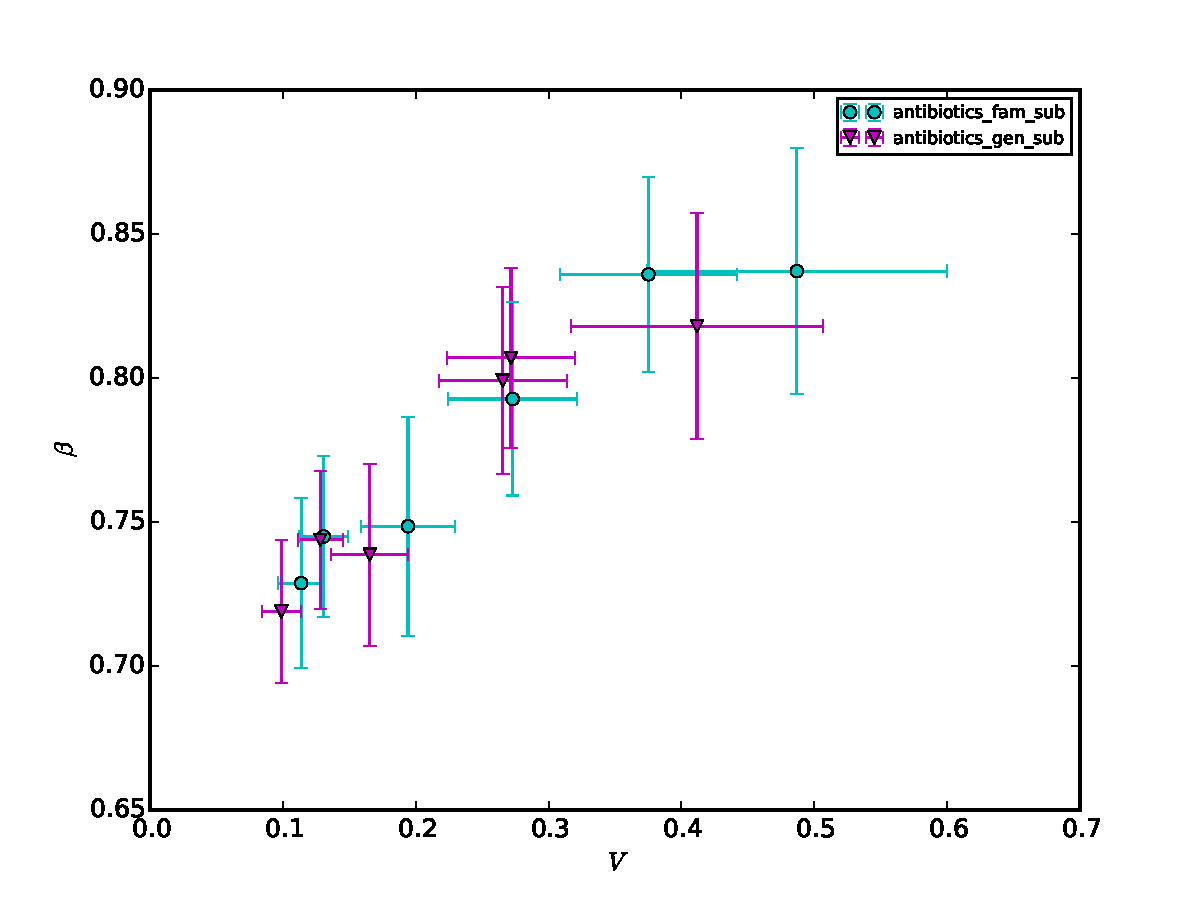
\includegraphics[width=0.5\textwidth]{results/taxalevel/sum_raw_16S.pdf}
  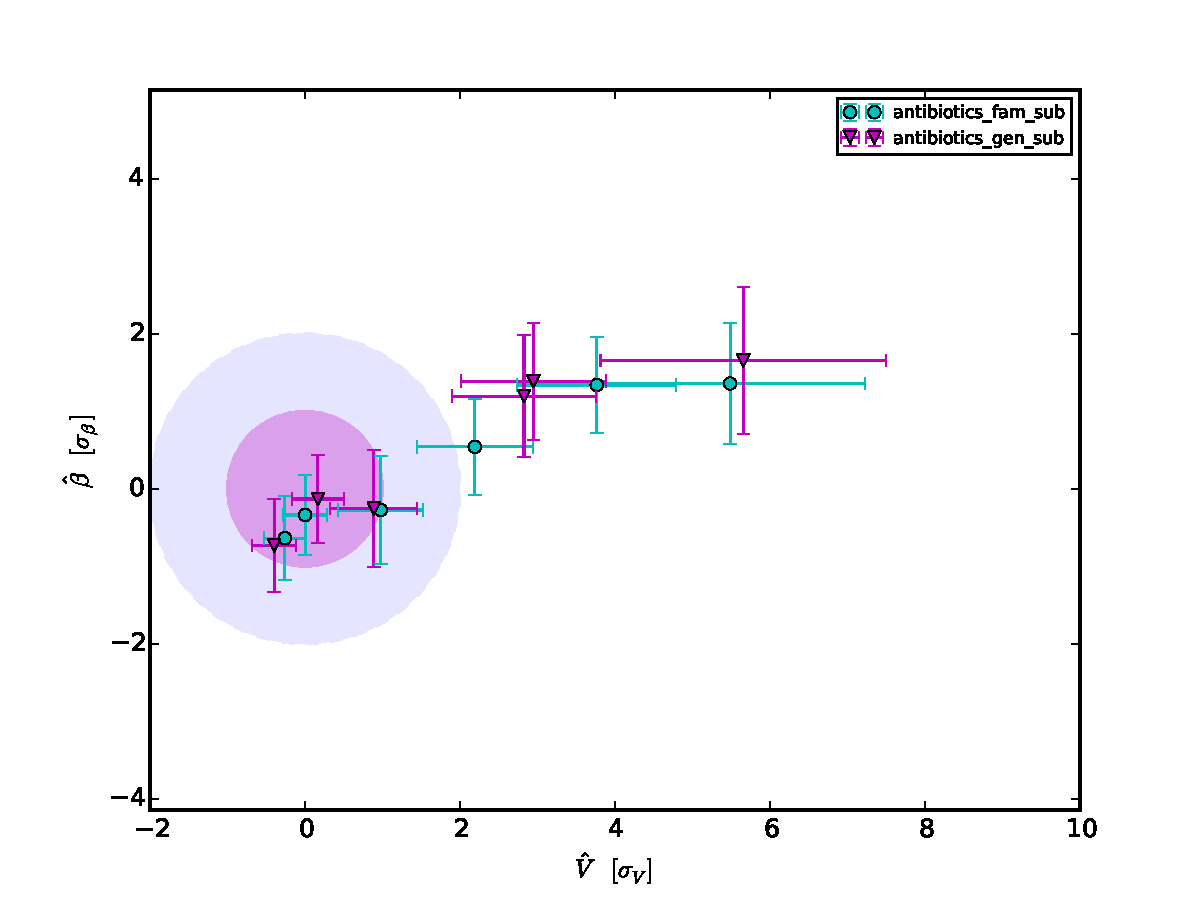
\includegraphics[width=0.5\textwidth]{results/taxalevel/sum_sta_16S.pdf}
  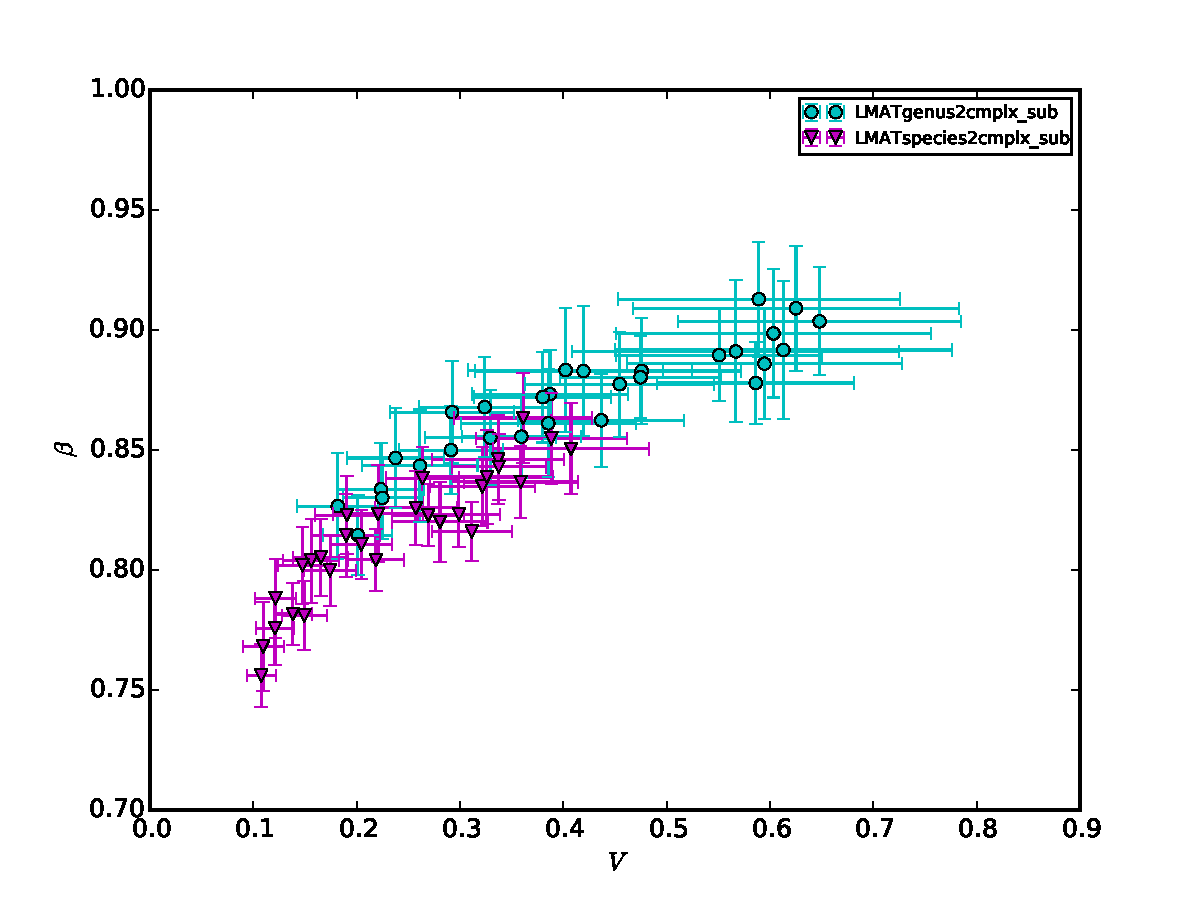
\includegraphics[width=0.5\textwidth]{results/taxalevel/sum_raw_SMS.pdf} 
  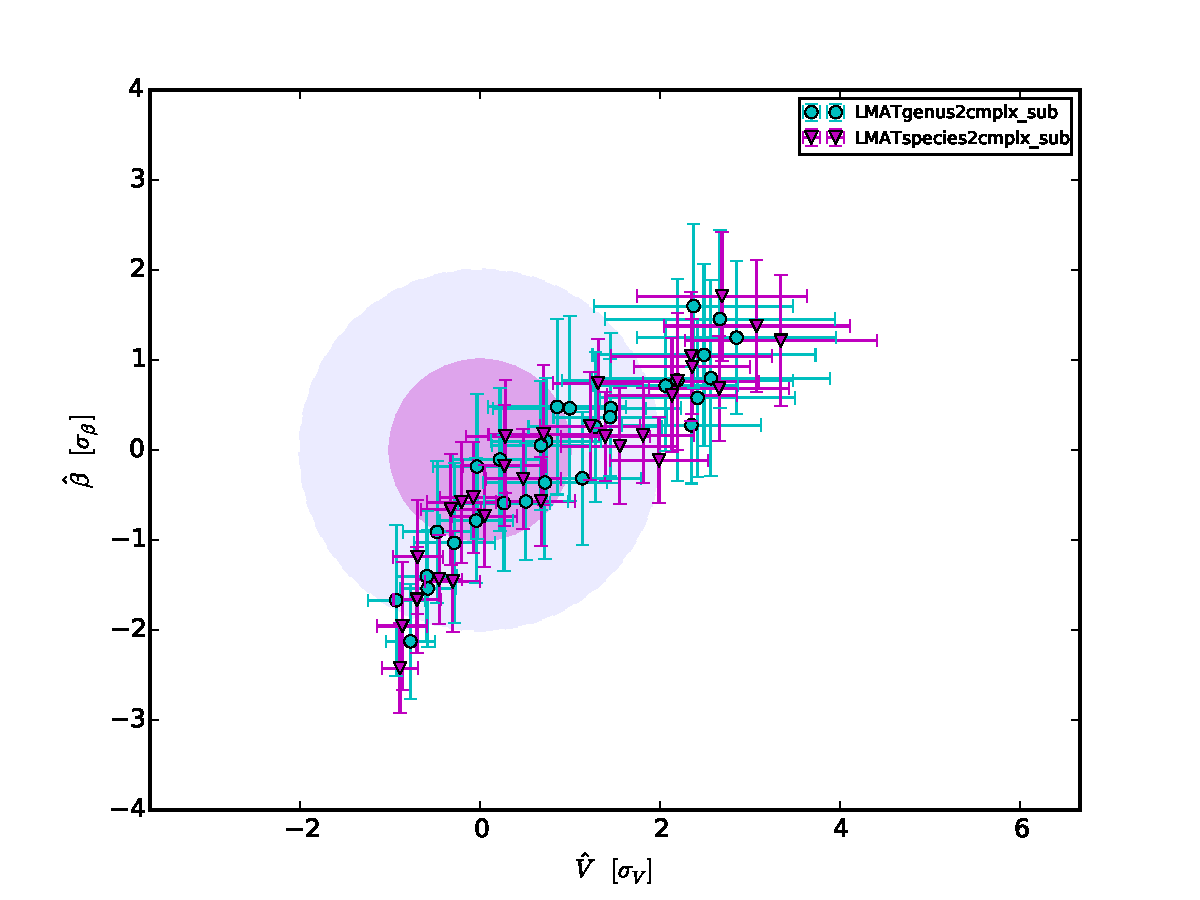
\includegraphics[width=0.5\textwidth]{results/taxalevel/sum_sta_SMS.pdf}
\caption{Overview of comparison of different approaches based on adjacent taxonomic levels using plots in the Taylor-parameters space. For 16S (former row of subfigures), the levels are family vs. genus, whereas for SMS (latter row of subfigures) levels are genus vs. species. The left column shows the raw results and the right column plots the standardized results (see Section \ref{sec:stan})}
\label{fig:taxlev1}
\end{figure}

\begin{figure} 
  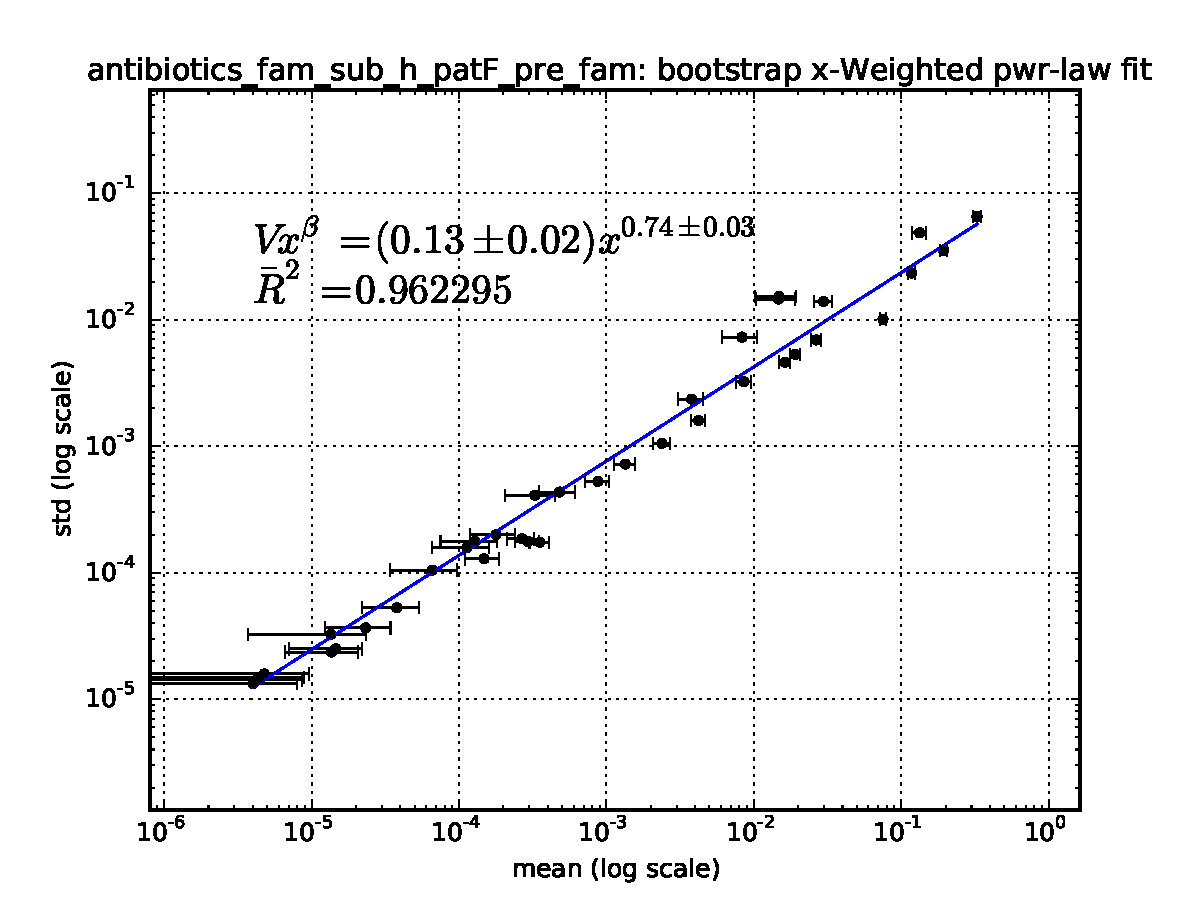
\includegraphics[width=0.5\textwidth]{results/taxalevel/xWb_fam_16S.pdf}
  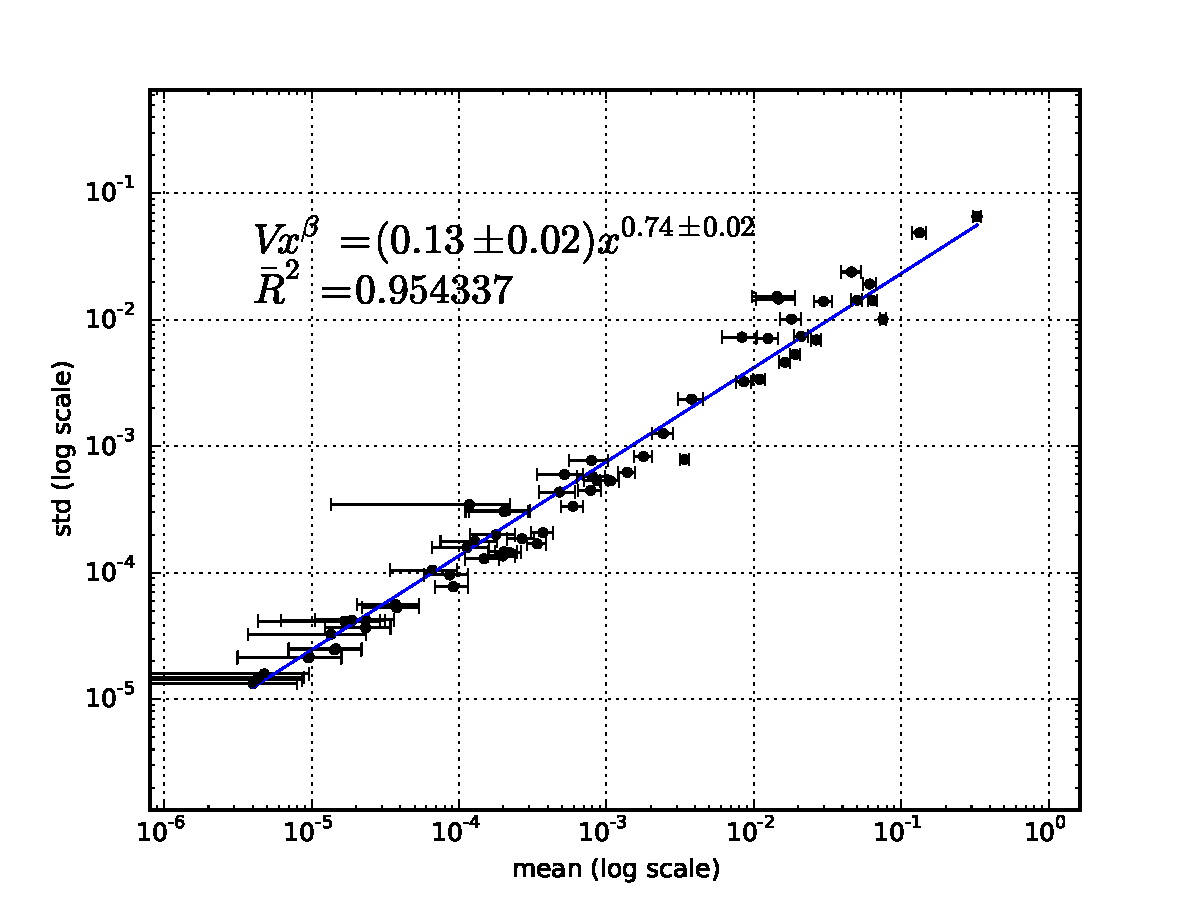
\includegraphics[width=0.5\textwidth]{results/taxalevel/xWb_gen_16S.pdf}
  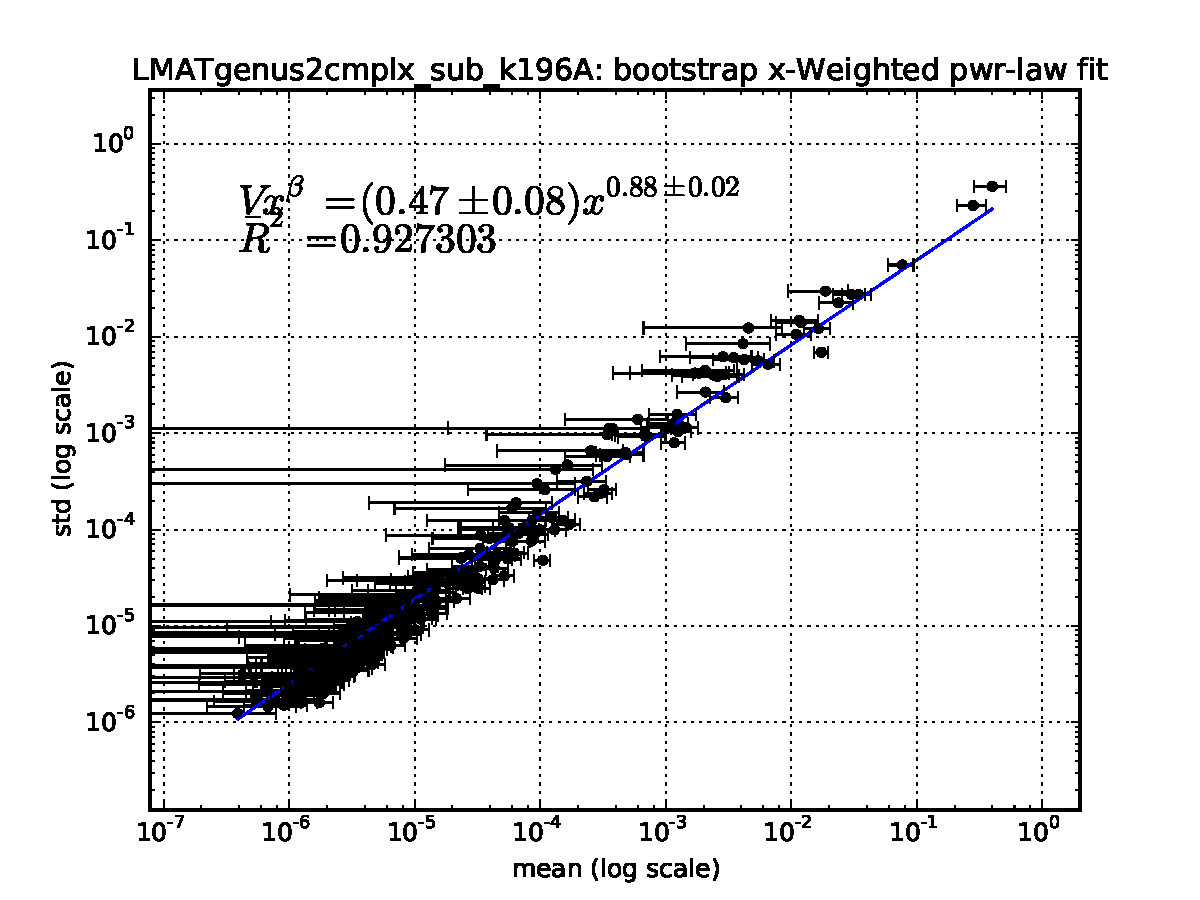
\includegraphics[width=0.5\textwidth]{results/taxalevel/xWb_gen_SMS.pdf}
  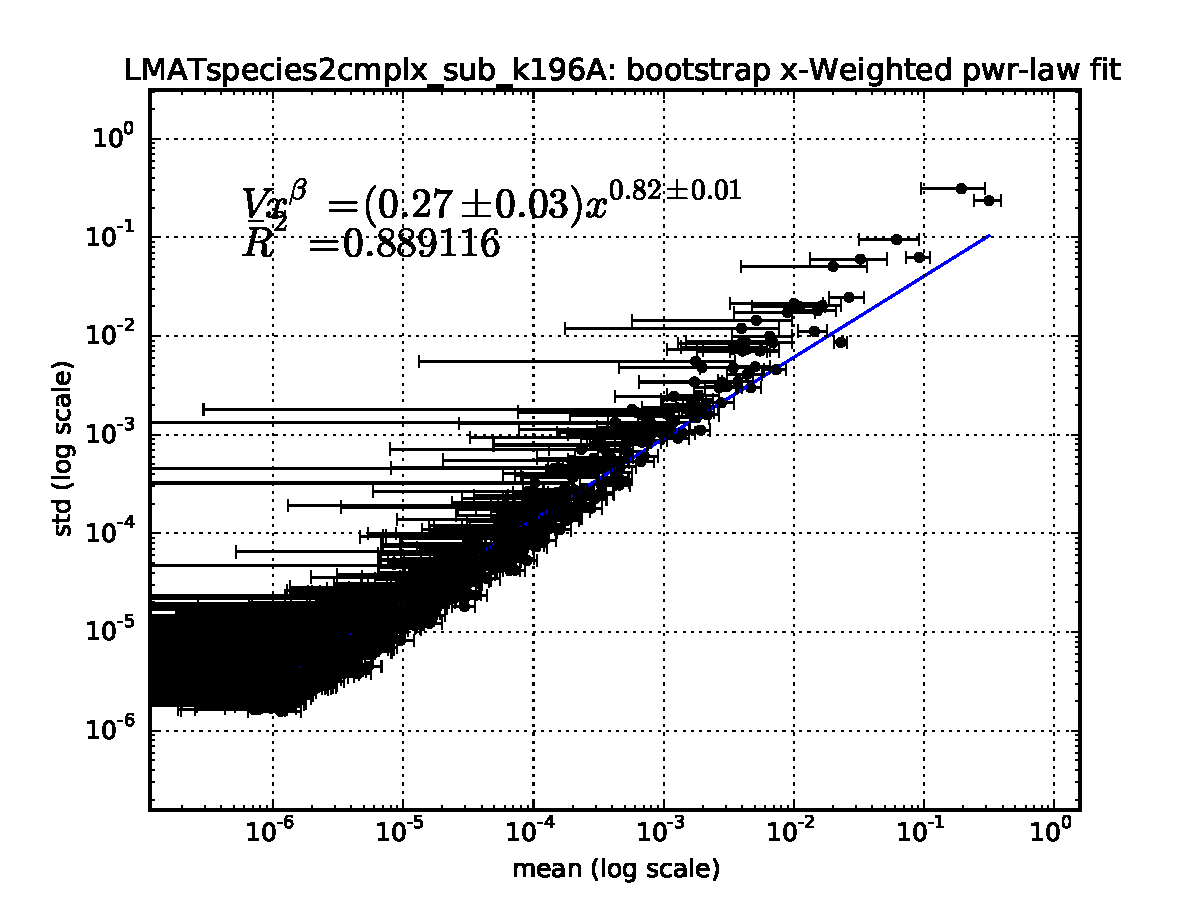
\includegraphics[width=0.5\textwidth]{results/taxalevel/xWb_spc_SMS.pdf}
\caption{Detail of comparison of different approaches based on adjacent taxonomic levels using plots of X-weighted power-law fits (see Section \ref{sec:X-w}). The former row of subfigures shows examples for 16S, whereas the latter row of subfigures plots examples for SMS. The left column shows results for the superior taxonomic level (family for 16S, genus for SMS), while the right column shows results for the inferior level (genus for 16S, specie for SMS).}
\label{fig:taxlev2}
\end{figure}

\begin{table} 
  \begin{center}
    \begin{tabular}{ccccccc}
	    \hline
		Metadata&V&$\beta$&$\bar{R}^2$&&V$_{st}$&$\beta_{st}$\\
		\hline
		A&$0.26 \pm 0.05$&$0.826 \pm 0.025$&$0.918$&&$3.1 \pm 0.9$&$1.2 \pm 0.6$\\
		A&$0.32 \pm 0.06$&$0.857 \pm 0.025$&$0.924$&&$4.4 \pm 1.1$&$2.0 \pm 0.6$\\
		A&$0.194 \pm 0.033$&$0.813 \pm 0.024$&$0.918$&&$1.9 \pm 0.6$&$0.9 \pm 0.6$\\
		A&$0.24 \pm 0.04$&$0.824 \pm 0.020$&$0.924$&&$2.7 \pm 0.7$&$1.2 \pm 0.5$\\
		A&$0.34 \pm 0.06$&$0.855 \pm 0.024$&$0.931$&&$4.7 \pm 1.1$&$1.9 \pm 0.6$\\
		A&$0.30 \pm 0.05$&$0.847 \pm 0.022$&$0.921$&&$3.9 \pm 1.0$&$1.7 \pm 0.5$\\
		A&$0.133 \pm 0.021$&$0.784 \pm 0.023$&$0.916$&&$0.7 \pm 0.4$&$0.2 \pm 0.6$\\
		A&$0.25 \pm 0.04$&$0.831 \pm 0.024$&$0.929$&&$3.0 \pm 0.8$&$1.4 \pm 0.6$\\
		\hline
		P&$0.23 \pm 0.05$&$0.804 \pm 0.035$&$0.885$&&$2.6 \pm 0.9$&$0.7 \pm 0.8$\\
		P&$0.097 \pm 0.018$&$0.705 \pm 0.031$&$0.891$&&$0.03 \pm 0.34$&$-1.6 \pm 0.7$\\
		P&$0.037 \pm 0.006$&$0.642 \pm 0.025$&$0.881$&&$-1.12 \pm 0.11$&$-3.1 \pm 0.6$\\
		P&$0.118 \pm 0.019$&$0.723 \pm 0.025$&$0.895$&&$0.4 \pm 0.4$&$-1.2 \pm 0.6$\\
		P&$0.17 \pm 0.04$&$0.78 \pm 0.04$&$0.842$&&$1.5 \pm 0.7$&$0.1 \pm 0.9$\\
		P&$0.123 \pm 0.020$&$0.757 \pm 0.026$&$0.914$&&$0.5 \pm 0.4$&$-0.4 \pm 0.6$\\
		P&$0.19 \pm 0.05$&$0.77 \pm 0.04$&$0.871$&&$1.8 \pm 0.9$&$-0.0 \pm 0.9$\\
		P&$0.121 \pm 0.020$&$0.736 \pm 0.027$&$0.921$&&$0.5 \pm 0.4$&$-0.9 \pm 0.6$\\
		P&$0.187 \pm 0.034$&$0.771 \pm 0.030$&$0.908$&&$1.8 \pm 0.7$&$-0.1 \pm 0.7$\\
		P&$0.097 \pm 0.015$&$0.735 \pm 0.025$&$0.922$&&$0.05 \pm 0.28$&$-0.9 \pm 0.6$\\
	   \hline
	   \hline
    \end{tabular}
  \end{center}
  \caption{Taylor parameters. Individuals with either animal-based (A) or plant-based (P) diets\cite{diet}. Previous to diet,  the population sampled is described by $\bar{V} = 0.09 \pm 0.05, \bar{\beta} = 0.77 \pm 0.04$.}
  \label{tab:diet}
\end{table}

 \begin{table} 
  \begin{center}
    \begin{tabular}{ccccccc}
	    \hline
		Metadata&V&$\beta$&$\bar{R}^2$&&V$_{st}$&$\beta_{st}$\\
		\hline
		Ab&$0.35 \pm 0.07$&$0.81 \pm 0.04$&$0.925$&&$4.3 \pm 1.4$&$1.3 \pm 0.9$\\
		Ab&$0.41 \pm 0.09$&$0.82 \pm 0.04$&$0.908$&&$5.6 \pm 1.8$&$1.6 \pm 0.9$\\
		Ab&$0.23 \pm 0.04$&$0.770 \pm 0.031$&$0.920$&&$2.1 \pm 0.8$&$0.5 \pm 0.7$\\
		Ab&$0.165 \pm 0.029$&$0.738 \pm 0.031$&$0.928$&&$0.9 \pm 0.6$&$-0.3 \pm 0.7$\\
		Ab&$0.34 \pm 0.06$&$0.812 \pm 0.032$&$0.936$&&$4.1 \pm 1.2$&$1.5 \pm 0.7$\\
		Ab&$0.26 \pm 0.05$&$0.798 \pm 0.033$&$0.931$&&$2.8 \pm 0.9$&$1.1 \pm 0.8$\\
	    \hline
	    \hline
    \end{tabular}
  \end{center}
  \caption{Taylor parameters for individuals taking antibiotics\cite{antibiotic}. Prior to antibiotics intake, the population sampled is described by $\bar{V} = 0.12 \pm 0.05, \bar{\beta} = 0.75 \pm 0.04$.}
  \label{tab:antibiotics}
\end{table}

\begin{table} 
  \begin{center}
    \begin{tabular}{ccccccc}
	    \hline
		Metadata&V&$\beta$&$\bar{R}^2$&&V$_{st}$&$\beta_{st}$\\
		\hline
		IBS&$0.204 \pm 0.034$&$0.739 \pm 0.029$&$0.916$&&$7.6 \pm 3.7$&$1.9 \pm 1.2$\\
		IBS&$0.35 \pm 0.05$&$0.793 \pm 0.023$&$0.935$&&$23.1 \pm 5.9$&$4.0 \pm 0.9$\\
	     \hline
	     \hline
    \end{tabular}
  \end{center}
  \caption{Taylor parameters for persons diagnosed with irritable bowel syndrome (IBS)\cite{IBS}. Healthy individuals sampled in this study are characterized by $\bar{V} = 0.134 \pm 0.009, \bar{\beta} = 0.691 \pm 0.025$.}
  \label{tab:IBS}
\end{table}

 \begin{table} 
  \begin{center}
    \begin{tabular}{ccccccc}
	    \hline
		Metadata&V&$\beta$&$\bar{R}^2$&&V$_{st}$&$\beta_{st}$\\
		\hline
		DH&$0.27 \pm 0.04$&$0.835 \pm 0.016$&$0.925$&&$0.2 \pm 0.4$&$-1.0 \pm 0.6$\\
		DH&$0.36 \pm 0.06$&$0.858 \pm 0.015$&$0.929$&&$1.1 \pm 0.6$&$-0.2 \pm 0.5$\\
		DH&$0.35 \pm 0.06$&$0.859 \pm 0.014$&$0.926$&&$1.0 \pm 0.5$&$-0.1 \pm 0.5$\\
		DH&$0.25 \pm 0.04$&$0.829 \pm 0.014$&$0.911$&&$0.0 \pm 0.4$&$-1.2 \pm 0.5$\\
		DH&$0.30 \pm 0.05$&$0.844 \pm 0.014$&$0.920$&&$0.5 \pm 0.4$&$-0.7 \pm 0.5$\\
		DH&$0.29 \pm 0.05$&$0.850 \pm 0.016$&$0.915$&&$0.4 \pm 0.5$&$-0.5 \pm 0.5$\\
		DH&$0.28 \pm 0.05$&$0.848 \pm 0.016$&$0.921$&&$0.3 \pm 0.5$&$-0.5 \pm 0.6$\\
		DH&$0.35 \pm 0.07$&$0.861 \pm 0.017$&$0.918$&&$0.9 \pm 0.6$&$-0.0 \pm 0.6$\\
		DH&$0.31 \pm 0.04$&$0.833 \pm 0.012$&$0.916$&&$0.6 \pm 0.4$&$-1.1 \pm 0.4$\\
		DH&$0.33 \pm 0.05$&$0.843 \pm 0.013$&$0.925$&&$0.8 \pm 0.5$&$-0.7 \pm 0.5$\\
		DH&$0.31 \pm 0.05$&$0.852 \pm 0.014$&$0.925$&&$0.6 \pm 0.5$&$-0.4 \pm 0.5$\\
		DH&$0.31 \pm 0.05$&$0.853 \pm 0.015$&$0.930$&&$0.6 \pm 0.5$&$-0.4 \pm 0.5$\\
		DH&$0.203 \pm 0.033$&$0.815 \pm 0.015$&$0.907$&&$-0.44 \pm 0.32$&$-1.7 \pm 0.5$\\
		\hline
    \end{tabular}
  \end{center}
  \caption{Taylor parameters for the healthy subject of the discordant twins\cite{kwashiorkor}. This table continues in Supplementary Table \ref{tab:DK}. The population of healthy twins is characterized by $\bar{V} = 0.25 \pm 0.10, \bar{\beta} = 0.863 \pm 0.028$.}
  \label{tab:DH}
\end{table}

\begin{table} 
  \begin{center}
    \begin{tabular}{ccccccc}
	    \hline
		Metadata&V&$\beta$&$\bar{R}^2$&&V$_{st}$&$\beta_{st}$\\
		\hline
		DK&$0.40 \pm 0.07$&$0.859 \pm 0.017$&$0.926$&&$1.5 \pm 0.7$&$-0.1 \pm 0.6$\\
		DK&$0.44 \pm 0.08$&$0.868 \pm 0.016$&$0.919$&&$1.8 \pm 0.8$&$0.2 \pm 0.6$\\
		DK&$0.196 \pm 0.031$&$0.819 \pm 0.014$&$0.916$&&$-0.50 \pm 0.30$&$-1.5 \pm 0.5$\\
		DK&$0.160 \pm 0.026$&$0.798 \pm 0.015$&$0.904$&&$-0.85 \pm 0.25$&$-2.3 \pm 0.5$\\
		DK&$0.30 \pm 0.05$&$0.845 \pm 0.014$&$0.924$&&$0.5 \pm 0.4$&$-0.6 \pm 0.5$\\
		DK&$0.23 \pm 0.04$&$0.834 \pm 0.014$&$0.908$&&$-0.1 \pm 0.4$&$-1.0 \pm 0.5$\\
		DK&$0.27 \pm 0.05$&$0.848 \pm 0.015$&$0.930$&&$0.2 \pm 0.4$&$-0.5 \pm 0.5$\\
		DK&$0.35 \pm 0.07$&$0.860 \pm 0.019$&$0.916$&&$1.0 \pm 0.7$&$-0.1 \pm 0.7$\\
		DK&$0.34 \pm 0.05$&$0.835 \pm 0.012$&$0.917$&&$0.9 \pm 0.5$&$-1.0 \pm 0.4$\\
		DK&$0.25 \pm 0.04$&$0.831 \pm 0.012$&$0.912$&&$0.0 \pm 0.4$&$-1.1 \pm 0.4$\\
		DK&$0.36 \pm 0.06$&$0.858 \pm 0.013$&$0.918$&&$1.1 \pm 0.5$&$-0.2 \pm 0.5$\\
		DK&$0.31 \pm 0.06$&$0.851 \pm 0.016$&$0.924$&&$0.6 \pm 0.6$&$-0.4 \pm 0.6$\\
		DK&$0.149 \pm 0.022$&$0.799 \pm 0.013$&$0.905$&&$-0.96 \pm 0.22$&$-2.2 \pm 0.5$\\
	    \hline
	    \hline
    \end{tabular}
  \end{center}
  \caption{Taylor parameters for the kwashiorkor part of the discordant twins\cite{kwashiorkor}. This is a continuation of Supplementary Table \ref{tab:DH}. The population of healthy twins is characterized by $\bar{V} = 0.25 \pm 0.10, \bar{\beta} = 0.863 \pm 0.028$.}
  \label{tab:DK}
\end{table}

\begin{table} 
  \begin{center}
    \begin{tabular}{ccccccc}
	    \hline
		Metadata&V&$\beta$&$\bar{R}^2$&&V$_{st}$&$\beta_{st}$\\
		\hline
		OW&$0.59 \pm 0.12$&$0.894 \pm 0.034$&$0.920$&&$6.6 \pm 2.0$&$2.6 \pm 1.0$\\
		OW&$0.22 \pm 0.04$&$0.830 \pm 0.030$&$0.904$&&$0.5 \pm 0.6$&$0.7 \pm 0.9$\\
		\hline
		OBI&$0.28 \pm 0.04$&$0.855 \pm 0.022$&$0.958$&&$1.5 \pm 0.6$&$1.4 \pm 0.6$\\
		OBI&$0.33 \pm 0.07$&$0.870 \pm 0.031$&$0.916$&&$2.4 \pm 1.1$&$1.9 \pm 0.9$\\
		\hline
		OBII&$0.223 \pm 0.032$&$0.823 \pm 0.023$&$0.938$&&$0.6 \pm 0.5$&$0.5 \pm 0.7$\\
		OBII&$0.208 \pm 0.029$&$0.844 \pm 0.022$&$0.935$&&$0.4 \pm 0.5$&$1.1 \pm 0.7$\\
		\hline
		OBIII&$0.34 \pm 0.05$&$0.855 \pm 0.025$&$0.943$&&$2.5 \pm 0.9$&$1.4 \pm 0.7$\\
		OBIII&$0.26 \pm 0.04$&$0.845 \pm 0.026$&$0.954$&&$1.1 \pm 0.7$&$1.2 \pm 0.8$\\
		OBIII&$0.33 \pm 0.06$&$0.870 \pm 0.027$&$0.908$&&$2.4 \pm 1.0$&$1.9 \pm 0.8$\\
		OBIII&$0.200 \pm 0.026$&$0.843 \pm 0.020$&$0.949$&&$0.2 \pm 0.4$&$1.1 \pm 0.6$\\
		OBIII&$0.30 \pm 0.05$&$0.846 \pm 0.026$&$0.929$&&$1.9 \pm 0.8$&$1.2 \pm 0.7$\\
		OBIII&$0.176 \pm 0.029$&$0.826 \pm 0.026$&$0.894$&&$-0.2 \pm 0.5$&$0.6 \pm 0.8$\\
		OBIII&$0.30 \pm 0.06$&$0.841 \pm 0.031$&$0.896$&&$1.8 \pm 0.9$&$1.0 \pm 0.9$\\
		OBIII&$0.28 \pm 0.04$&$0.857 \pm 0.025$&$0.941$&&$1.5 \pm 0.7$&$1.5 \pm 0.7$\\
		OBIII&$0.122 \pm 0.018$&$0.822 \pm 0.024$&$0.930$&&$-1.05 \pm 0.30$&$0.5 \pm 0.7$\\
		\hline
		OBIIId&$0.47 \pm 0.08$&$0.872 \pm 0.023$&$0.945$&&$4.7 \pm 1.3$&$1.9 \pm 0.7$\\
		OBIIId&$0.38 \pm 0.06$&$0.846 \pm 0.023$&$0.951$&&$3.2 \pm 1.0$&$1.2 \pm 0.7$\\
		OBIIId&$0.36 \pm 0.06$&$0.842 \pm 0.022$&$0.954$&&$2.9 \pm 0.9$&$1.1 \pm 0.6$\\
	    \hline
	    \hline
    \end{tabular}
  \end{center}
  \caption{Taylor parameters for individuals with different degrees of overweight and obesity\cite{LEA}. Healthy people in this study, whom were not obese, are characterized by $\bar{V} = 0.19 \pm 0.06, \bar{\beta} = 0.806 \pm 0.034$.}
  \label{tab:LEA}
\end{table}


\subsection*{ComplexCruncher}

A complete software framework, named 'ComplexCruncher', has been engineered to support the analysis of the dynamics of ranking processes in complex systems. Although the software was devised with a clear bias towards metagenomics, it is general enough to be able to cope with a ranking process in any complex system. Implemented in Python using well-known open-source community software, the software solution is composed of two parts that can be used together or apart: a web-based graphic front-end connected to a database, and a computing kernel. Used together, this software enables other users to reproduce our results easily and, furthermore, upload and analyse their own data or experiment with the preloaded metagenomics data sets.

`ComplexCruncher WebPortal' (CCWebPortal) is a web platform designed to allow the user to interact with a data repository of selected and well-documented metagenomics data sources. Through a few simple steps, the user can perform advanced searches on the complete set of records in the metagenomics repository.  The web application provides advanced filters that allow the user to reduce the search to a small set of interest. After this first step, the user can refine the search and discard those records that do not meet certain requirements.

The web application allows calculations to be done directly by the stable release of the \CC\ computing kernel. At the end of the calculations, the results are displayed to the user on the same browser which runs the web application. Then, the user can interact over the series of generated graphics thus allowing flexible comparison among them. In addition, CCWebPortal enables direct download of generated data (plots, spreadsheets, etc). The web application generates a report file summarizing all the results in PDF format. If the user has login permissions, CCWebPortal enables the option of insert new database records in addition to editing and deleting existing ones.

CCWebPortal is a web application that runs on current versions of many browsers. Additional software is not needed and only requires javaScript to be enabled on the browser to run applications. 
CCWebPortal is implemented following the client$-$server distributed programming model, where the javaScript client application connects to a remote server that enables the execution of calculations and transactions through a centralized database management system. A set of relational tables allows the structuring of the metagenomics repository to establish relationships between records. Thus the search and information threshing is optimized for queries launched from the client interface. Access to the database on the server is implemented through Django framework, an open-source framework written in Python using the model-view-controller (MVC) architectural pattern for implementing user interfaces.

The effective data analysis has been performed with a Python tool developed from scratch to more than 4200 lines of code. Implemented following the Object Oriented Programming, paradigm, this software is the back-end of the website described above. However, it could be run as an independent piece of software since it is built as a Python package provided with a command-line front-end (\CC.py). Once installed, the tool can be run interactively but also in automatic mode, which uses parallel computation to speed up the analysis of several data sources. 

\CC\ performs the power-law fit described in the \emph{Blumm, N. et al.} paper, but by fitting the best model, i.e. choosing between fitting a power-law using linear regression versus nonlinear regression\cite{ecology}. In the power-law fit plots we also show the generalized coefficient of determination computed for continuous models\cite{genR2,disR2}.

\subsection*{Un-weighted power-law fit}\label{sec:unw}

\subsubsection*{Fitting the best model}

As already mentioned, to choose between fitting power laws ($y=Vx^\beta$) using linear regression on log-transformed (LLR) data versus non-linear regression (NLR), we mainly follow \emph{General Guidelines for the Analysis of Biological Power Laws}\cite{ecology}. It consists of the following three steps:
\begin{enumerate}
    \item Determining the appropriate error structure by likelihood analysis.
    \begin{enumerate}
        \item Fit the Non-Linear Regression (NLR) model and obtain $V_\text{NLR}$, $\beta_\text{NLR}$ and $\sigma_\text{NLR}^2$.
        \item Calculate the loglikelihood that the data ($n$ is sample size) are generated from a normal distribution with additive error:
        \begin{itemize}
            \item The likelihood of a normal distribution is: 
            \begin{linenomath}
            $$\mathcal{L}_\text{norm} = \prod_{i=1}^n\left[\frac{1}{\sqrt{2\pi\sigma^2_\text{NLR}}}\;\exp{\left(-\frac{\left(y_i-V_\text{NLR}x_i^{\beta_\text{NLR}}\right)^2}{2\sigma^2_\text{NLR}}\right)}\right]$$
            \end{linenomath}
            \item So, the loglikelihood of a normal distribution is:
            \begin{eqnarray*}
                \log\mathcal{L}_\text{norm} &=& -\frac{n}{2}\log\left|2\pi\sigma^2_\text{NLR}\right| - \frac{1}{2\sigma^2_\text{NLR}}\underbrace{\sum_{i=1}^n\left(y_i-V_\text{NLR}x_i^{\beta_\text{NLR}}\right)^2}_{\mathrm{RSS
                }_\text{NLR}}\\
                &=& -\frac{n}{2}\log\left|2\pi\sigma^2_\text{NLR}\right|-\frac{\mathrm{RSS}_\text{NLR}}{2\sigma^2_\text{NLR}}
            \end{eqnarray*}
        \end{itemize}
        \item Calculate the \emph{corrected Akaike's Information Criterion} for the NLR model:
		\begin{linenomath}
        $$\mathrm{AIC_{c_{NLR}}} = 2k - 2\log\mathcal{L}_\text{norm} + \frac{2k(k+1)}{n-k-1}$$
		\end{linenomath}
        \item Fit the Log-transformed Linear Regression (LLR) model and obtain $V_\text{LLR}$, $\beta_\text{LLR}$ and $\sigma_\text{LLR}^2$.
        \item Calculate the loglikelihood that the data ($n$ is sample size) are generated from a lognormal distribution with multiplicative error:
        \begin{itemize}
            \item The likelihood of a lognormal distribution is: 
            \begin{linenomath}
            $$\mathcal{L}_\text{logn} = \prod_{i=1}^n\left[\frac{1}{y_i\sqrt{2\pi\sigma^2_\text{LLR}}}\;\exp{\left(-\frac{\left(\log|y_i|-\log|V_\text{LLR}|-\beta_\text{LLR}\log|x_i|\right)^2}{2\sigma^2_\text{LLR}}\right)}\right]$$
            \end{linenomath}
            \item So, the loglikelihood of a lognormal distribution is: 
            \begin{eqnarray*}
                \log\mathcal{L}_\text{logn} &=& -\frac{n}{2}\log\left|2\pi\sigma^2_\text{LLR}\right| - \sum_{i=1}^n\log|y_i| -\\
                &&\qquad-\frac{1}{2\sigma^2_\text{LLR}}\underbrace{\sum_{i=1}^n\left(\log|y_i|-\log|V_\text{LLR}|-\beta_\text{LLR}\log|x_i|\right)^2}_{\mathrm{RSS
                }_\text{LLR}}\\
                &=& -\frac{n}{2}\log\left|2\pi\sigma^2_\text{LLR}\right| - \frac{\mathrm{RSS}_\text{LLR}}{2\sigma^2_\text{LLR}} - \sum_{i=1}^n\log|y_i|
            \end{eqnarray*}
        \end{itemize}
        \item Calculate the \emph{corrected Akaike's Information Criterion} for the LR model: 
        	\begin{linenomath}
        	$$\mathrm{AIC_{c_{LLR}}} = 2k - 2\log\mathcal{L}_\text{logn} + \frac{2k(k+1)}{n-k-1}$$
			\end{linenomath}
    \end{enumerate}
    \item Compare $\mathrm{AIC_{c_{NLR}}}$ with $\mathrm{AIC_{c_{LLR}}}$:
    \begin{itemize}
        \item If $\mathrm{AIC_{c_{NLR}}} - \mathrm{AIC_{c_{LLR}}} < -2$, the assumption of normal error is favoured compared to lognormal error, so proceed with the results obtained from the NLR fit.
        \item If $\mathrm{AIC_{c_{NLR}}} - \mathrm{AIC_{c_{LLR}}} > 2$, the assumption of lognormal error is favoured compared to normal error, so proceed with the results obtained from the LLR fit.
        \item If $\left|\mathrm{AIC_{c_{NLR}}} - \mathrm{AIC_{c_{LLR}}}\right| \leq 2$, no model is favoured, so proceed with model averaging:
        \begin{eqnarray*}
            B_\text{av} &=& w_\text{NLR}V_\text{NLR} + w_\text{LLR}V_\text{LLR} \\
            \beta_\text{av} &=& w_\text{NLR}\beta_\text{NLR} + w_\text{LLR}\beta_\text{LLR}
        \end{eqnarray*}
        where: 
        \begin{eqnarray*}
            w_\text{NLR} &=& \frac{1}{1+\mathrm{e}^{\frac{1}{2}\left(\mathrm{AIC_{c_{NLR}}}-\mathrm{AIC_{c_{LLR}}}\right)}} \\
            w_\text{LLR} &=& \frac{1}{1+\mathrm{e}^{\frac{1}{2}\left(\mathrm{AIC_{c_{LLR}}}-\mathrm{AIC_{c_{NLR}}}\right)}}
        \end{eqnarray*}
        which are obtained to fulfill the next condition: $w_\text{NLR} + w_\text{LLR} = 1$. The CIs for $B_\text{av}$ and $\beta_\text{av}$ are to be generated by ordinary bootstrapping\footnote{\CC\ has available the next bootstrapping alternatives\cite{boot}: ordinary, ``Resampling Residuals'' method, ``Wild'' method, and ``Monte-Carlo'' method.}.      
    \end{itemize}
    \item Assess the validity of the underlying statistical assumptions with diagnostic plots because while it is rare for all the assumptions to be fully satisfied by real-life data sets, major violations indicate the lack of appropriateness of the model and, thus, the potential invalidity of the results.
\end{enumerate}

\subsubsection*{Calculating the coefficient of determination}

We think the best approach in this situation is to apply the generalized $R^2$ that, for continuous models, was defined as\cite{genR2}:
\begin{linenomath}
$$ R^2 = 1 - \left(\frac{\mathcal{L}(0)}{\mathcal{L}(\hat\theta)}\right)^{\!\!\frac{2}{n}} $$
\end{linenomath}
where $\mathcal{L}(\hat\theta)$ and $\mathcal{L}(0)$  denote the likelihoods of the fitted and the ``null'' model, respectively, and $n$ is the sample size. In terms of the loglikelihoods, the generalized coefficient of determination would be:
\begin{linenomath}
$$ R^2 = 1 - \mathrm{e}^{-\frac{2}{n}\left(\log\mathcal{L}(\hat\theta)-\log\mathcal{L}(0)\right)} $$
\end{linenomath}
We have the likelihoods calculated from the previous section, but what about the ``null'' models? We understand that they are the models with only the intercept. So for the Gaussian additive error model:
\begin{linenomath}
$$\mathcal{L}_\text{norm}(0) = \prod_{i=1}^n\left[\frac{1}{\sqrt{2\pi\sigma^2_\text{NLR0}}}\;\exp{\left(-\frac{\left(y_i-\bar y\right)^2}{2\sigma^2_\text{NLR0}}\right)}\right]$$
\end{linenomath}
So:
\begin{eqnarray*}
\log\mathcal{L}_\text{norm}(0) &=& -\frac{n}{2}\log\left|2\pi\sigma^2_\text{NLR0}\right| - \frac{1}{2\sigma^2_\text{NLR0}}\sum_{i=1}^n\left(y_i-\bar y\right)^2\\
 &=& -\frac{n}{2}\left(\log\left|2\pi\sigma^2_\text{NLR0}\right| + 1 \right)
\end{eqnarray*}
since $\sigma^2_\text{NLR0}=\frac{1}{n}\sum\left(y_i-\bar y\right)^2=\frac{1}{n}\mathrm{TSS}_\text{NLR}$. Now, coming back to the coefficient of determination, we have:
\begin{eqnarray*}
R^2_\text{NLR} &=& 1 - \mathrm{e}^{\frac{2}{n}\left(\log\mathcal{L}_\text{NLR}(0)-\log\mathcal{L}_\text{NLR}(\hat\theta)\right)} = 1 - \exp{\left(\frac{\log(\mathrm{RSS}_\text{NLR})}{\log(\mathrm{TSS}_\text{NLR})}\right)}
 =\\ &=& 1 - \frac{\mathrm{RSS}_\text{NLR}}{\mathrm{TSS}_\text{NLR}} =
 1 - \frac{\sum_{i=1}^n\left(y_i-V_\text{NLR}x_i^{\beta_\text{NLR}}\right)^2}{\sum_{i=1}^n\left(y_i-\bar y\right)^2}
\end{eqnarray*}
recovering the traditional expression for $R^2$. Using the same approach for calculating $R^2_\text{LLR}$, then:
\begin{linenomath}
$$\mathcal{L}_\text{logn}(0) = \prod_{i=1}^n\left[\frac{1}{y_i\sqrt{2\pi\sigma^2_\text{LLR0}}}\;\exp{\left(-\frac{\left(\log|y_i|-\log|B_\text{LLR0}|\right)^2}{2\sigma^2_\text{LLR0}}\right)}\right]$$
\end{linenomath}
So:
\begin{eqnarray*}
\log\mathcal{L}_\text{logn}(0) &=& -\frac{n}{2}\log\left|2\pi\sigma^2_\text{LLR0}\right| - \frac{1}{2\sigma^2_\text{LLR0}}\sum_{i=1}^n\left(\log|y_i|-\overline{\log|y|}\right)^2 - \sum_{i=1}^n\log|y_i|\\
 &=& -\frac{n}{2}\left(\log\left|2\pi\sigma^2_\text{LLR0}\right| + 1 \right) - \sum_{i=1}^n\log|y_i|
\end{eqnarray*}
since $\sigma^2_\text{LLR0}=\frac{1}{n}\sum\left(\log|y_i|-\overline{\log|y|}\right)^2=\frac{1}{n}\mathrm{TSS}_\text{logn}$. Again, recalling the expression for the generalized coefficient of determination, we have:
\begin{eqnarray*}
R^2_\text{LLR} &=& 1 - \mathrm{e}^{\frac{2}{n}\left(\log\mathcal{L}_\text{LLR}(0)-\log\mathcal{L}_\text{LLR}(\hat\theta)\right)} = 1 - \exp{\left(\frac{\log(\mathrm{RSS}_\text{LLR})}{\log(\mathrm{TSS}_\text{LLR})}\right)}
 =\\ &=& 1 - \frac{\mathrm{RSS}_\text{LLR}}{\mathrm{TSS}_\text{LLR}} =
 1 - \frac{\sum_{i=1}^n\left(\log|y_i|-\log|V_\text{LLR}|-\beta_\text{LLR}\log|x_i|\right)^2}{\sum_{i=1}^n\left(\log|y_i|-\overline{\log|y|}\right)^2}
\end{eqnarray*}


\subsection*{X-weighted power-law fit}\label{sec:X-w}

When fitting the power-law of std vs. mean, we can take into account that every mean has uncertainty and estimate it for a sample size $n$ by the SEM (\emph{Standard Error of the Mean}):
\begin{linenomath}
$$ \mathrm{SEM} = \frac{s}{\sqrt{n}}$$
\end{linenomath}
where $s$ is the sample standard deviation. So, the vector of weights is computed with:
\begin{linenomath}
$$ \mathbf{w} = \frac{1}{\overrightarrow{\mathrm{SEM}}} = \frac{\sqrt{\mathbf{n}}}{\mathbf{s}}$$
\end{linenomath}

Here, the uncertainties affect the independent variable, so the fit is not so trivial as a Y-weighted fit, where the uncertainties affect the dependent variable. A standard approach to do this fit is: a) invert your variables before applying the weights, b) then perform the weighted fit, and finally, c) revert the inversion. This method is deterministic, but the approximate solution worsens with smaller $R^2$. For comparison, we develop a stochastic method by using a bootstrapping-like strategy that avoids the inversion and is applicable regardless of $R^2$. Both methods, detailed below, are implemented in \CC.

\subsubsection*{Method 1: By inverting the data}

In the case of the log-LR model, we have:
\begin{linenomath}
$$\log y = \log V + \beta\log x \quad\rightarrow\quad \underbrace{\log x}_{\tilde y} = \overbrace{-\frac{1}{\beta}\log V}^{b} + \overbrace{\frac{1}{\beta}}^{m}\underbrace{\log y}_{\tilde x}$$ 
\end{linenomath}
where $m$ determines the slope or gradient of the fitted line, and $b$ determines the point at which the line crosses the y-axis, otherwise known as the y-intercept. Once the model is fitted, the original parameters can be retrieved easily:
\begin{eqnarray*}
\beta &=& \frac{1}{m} \\
V &=& \mathrm{e}^{-\beta b} = \mathrm{e}^{-\frac{b}{m}}
\end{eqnarray*}
Their respective uncertainties are to be obtained using \emph{error propagation}:
\begin{eqnarray*}
    \sigma_\beta &=& \left|\frac{\mathrm{d}\beta}{\mathrm{d}m}\right|\sigma_m \quad=\quad \frac{1}{m^2}\;\sigma_m \\
    \sigma_V &=& \sqrt{\left(\frac{\partial V}{\partial b}\right)^{\!\!2}\sigma_b^2 +
      \left(\frac{\partial V}{\partial m}\right)^{\!\!2}\sigma_m^2} \quad=\quad
      \frac{1}{m}\;\mathrm{e}^{-\frac{b}{m}}\,\sqrt{\sigma_b^2 + \frac{b^2}{m^2}\;\sigma_m^2} 
\end{eqnarray*}

\subsubsection*{Method 2: Bootstrapping-like strategy}

The basic idea of bootstrapping is that inference about a population from sample data (sample $\rightarrow$ population) can be modeled by resampling the sample data and performing inference on (resample $\rightarrow$ sample). To adapt this general idea to our problem, we resample the x-data array using its errors array. That is, for each replicate, a new x-data array is computed based on:
\begin{linenomath}
$$x^*_i = x_i + v_i$$
\end{linenomath}
where $v_i$ is a Gaussian random variable with mean $\mu_i=0$ and standard deviation $\sigma_i=\mathrm{SEM}_i$, as defined previously in this supplementary material. For each replicate a complete un-weighted power-law fit is performed, as described in the previous section. It is worth mentioning that each replicate is filtered to avoid values of $x^*_i$ under \emph{eps} (obtained by \texttt{np.finfo(np.double).eps}) in order to keep away from the error of getting log of negatives or zero during the fit.

We devised and implemented a multi-step algorithm to estimate the fit parameters that finishes when a relative error of less than $10^{-4}$ is achieved. It also ends if the number of steps reaches $100$ to avoid too much time lapse, to prevent any pathologic numeric case which, in fact, we still have not detected in all the data sets analyzed.

In the previous version of the algorithm, for each step, the method generated $10$ replicates for each x-data point, in other words, it was computing the fit for $10$ times the length of the x-data array replicates, with a maximum of $10000$ fits per step. Nevertheless, we found that such an approach depending on the length of the x-data array did not perform better, so we decided to simplify the method and fix the number of fits per step in $100$. This latter approach improved the performance. 

The parameters of the X-weighted fit are then estimated by averaging through all the replicate fits performed, and their errors are estimated by computing the standard deviation also for all the fits. At the end of each step, the relative error is calculated by comparing the fit parameters estimation in the last step with the previous one.

Finally, both the coefficient of determination of the fit and the coefficient of correlation between the fit parameters are estimated by averaging.

\subsection*{Rank Stability Index (RSI)}\label{sec:RSI}

The Rank Stability Index is shown as a percentage in a separate bar on the right of the rank matrix plot provided by \CC. The RSI is strictly $1$ for an element whose range never changes over time, and is strictly $0$ for an element whose rank oscillates between the extremes from time to time. So, RSI is calculated, per element, as $1$ less the quotient of the number of true rank hops taken between the number of maximum possible rank hops, all powered to $p$:
\begin{linenomath}
$${\rm RSI} = \left(1-\frac{\text{true rank hops}}{\text{possible rank hops}}\right)^p = \left(1-\frac{D}{(N-1)(t-1)}\right)^p$$
\end{linenomath}
where $D$ is the total of rank hops taken by the studied element, $N$ is the number of elements that have been ranked, and $t$ is the number of time samples. The power index $p$ is arbitrarily chosen to increase the resolution in the stable region; the value in the current version of the code is $p=4$. 

As an example of this ``zooming'' effect in the stable region, to match a linear ($p=1$) RSI of 0.9 to a powered one of 0.1, we should select $p=21.8543$. An alternative way to obtain this effect and exactly map a linear RSI of 0.9 to a non-linear RSI (${\rm RSI'}$) of 0.1, is by applying the following function:
\begin{linenomath}
$${\rm RSI'} = \frac{10^{10\left(1-\frac{D}{(N-1)(t-1)}\right)}-1}{10^{10}-1} \approx 10^{-10\left(\frac{D}{(N-1)(t-1)}\right)}$$
\end{linenomath}
where the approximation is valid because $10^{10}\gg 1$ but, the small price to pay for it is that, in the worst instability case, the ${\rm RSI'}$ would not be strictly $0$ but $10^{-10}$.

The colour code of the RSI percentage text in the rank plot of \CC\ is chosen following the first condition satisfied from those shown in Table \ref{tab:RSI} (see page \pageref{tab:RSI}). 

\begin{table}
  \begin{center}
    \begin{tabular}{ccc}
    \hline
    Case  &  Condition  &  Colour  \\
    \hline
    1  &  $1\ge{\rm RSI}>0.99$  & \textcolor{blue}{blue}  \\ 
    2  & ${\rm RSI}>0.90$  &  \textcolor{green}{green}  \\
    3  &  ${\rm RSI}>0.75$  &  \textcolor{orange}{orange} \\
    4  &  ${\rm RSI}>0.25$  &  \textcolor{red}{red} \\
    5  &  $0.25\ge{\rm RSI}\ge0$  &  \bfseries{black}  \\
    \hline
    \end{tabular}
  \end{center}
  \caption{Colour code of the RSI percentage text shown in rank plots, following the first condition satisfied.}
  \label{tab:RSI}
\end{table}

\subsection*{\CC\ output}
In the previous sections, we have discussed details about the methods used in \CC. In this section we review the output from the package, which aims at summarizing the as yet undescribed functionality. 

\subsubsection*{Fit Plots}
Both for the unweighted fit (detailed in the section \ref{sec:unw}) and for the X-weighted fit (detailed in the section \ref{sec:X-w}), two plots are generated: the former with logarithmic scale, the latter with lineal scale. Figure \ref{fig:unwFit} shows an example of the unweighted fit plots and Figure \ref{fig:X-wFit} does the same with the X-weighted fit plots. Additionally, for the unweighted fit, a complete residues analysis is performed, and a 4-in-1 figure is generated as shown in Figure \ref{fig:unwRes}, corresponding to the fit of Figure \ref{fig:unwFit}. Among other tests, it allows to check for normality and homoscedasticity of the residues.

\begin{figure}
	\centering
	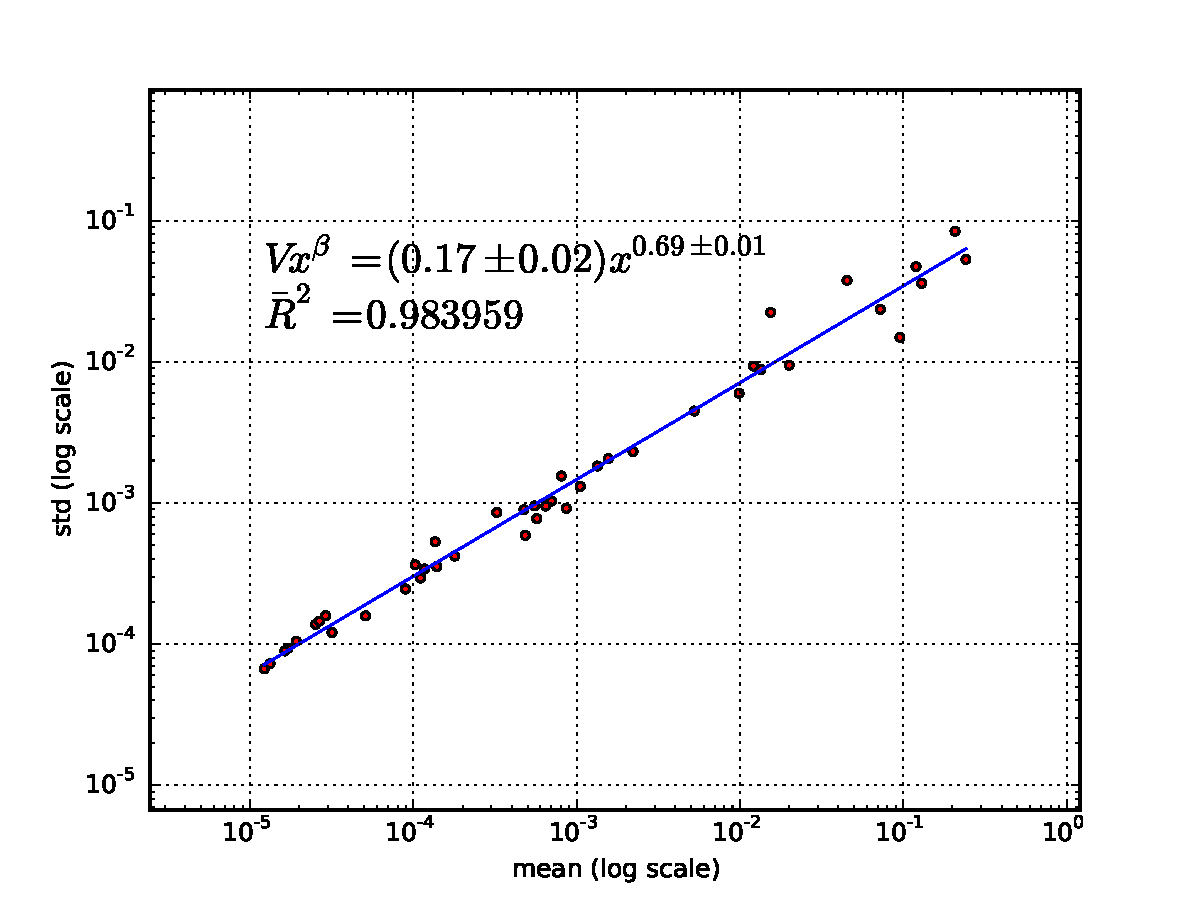
\includegraphics[width=0.8\textwidth]{results/fits/IBS_h_A_amplicons_family_stdVSmean_LLR_LOG.pdf}
	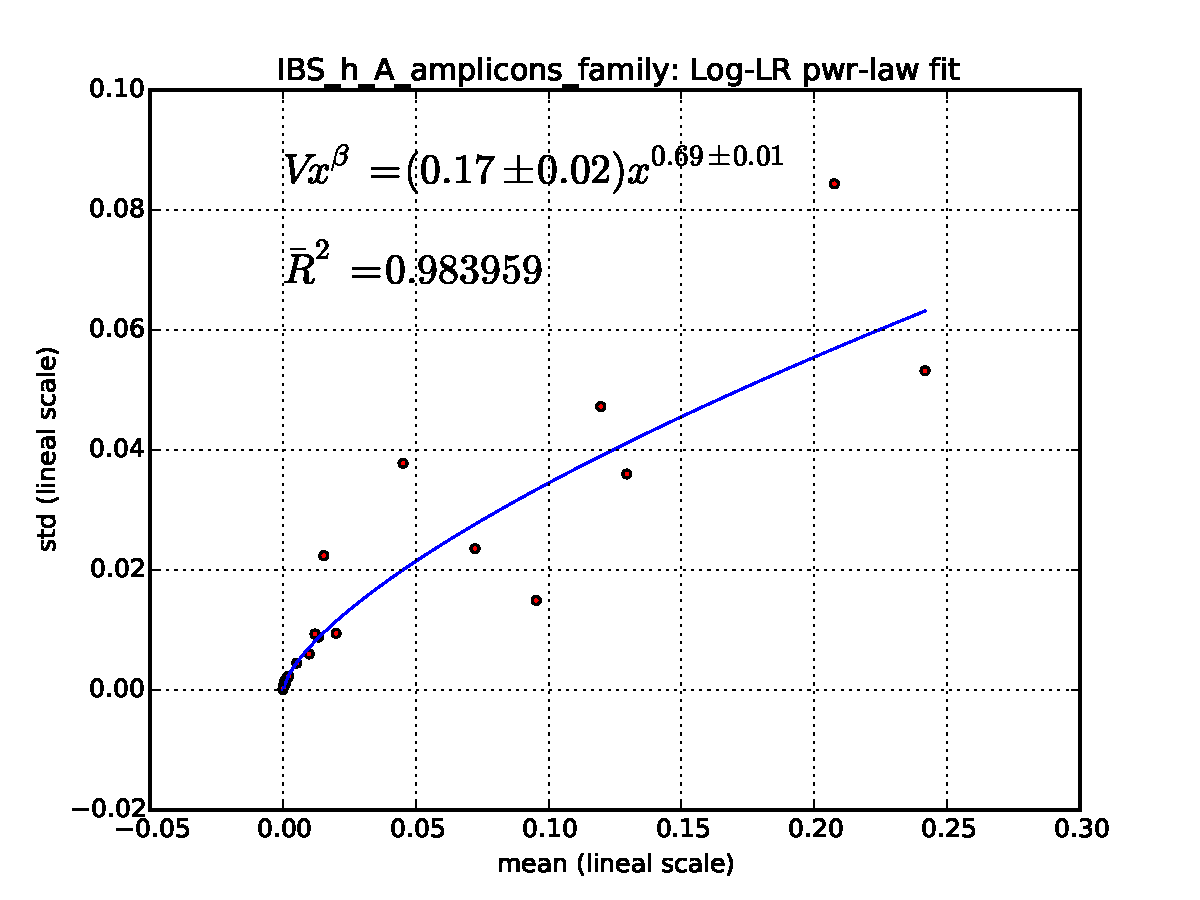
\includegraphics[width=0.8\textwidth]{results/fits/IBS_h_A_amplicons_family_stdVSmean_LLR_LIN.pdf}
	\caption{Example of unweighted fit, shown both in logarithmic and lineal scale plots}
	\label{fig:unwFit}
\end{figure}

\begin{figure}
	\centering
	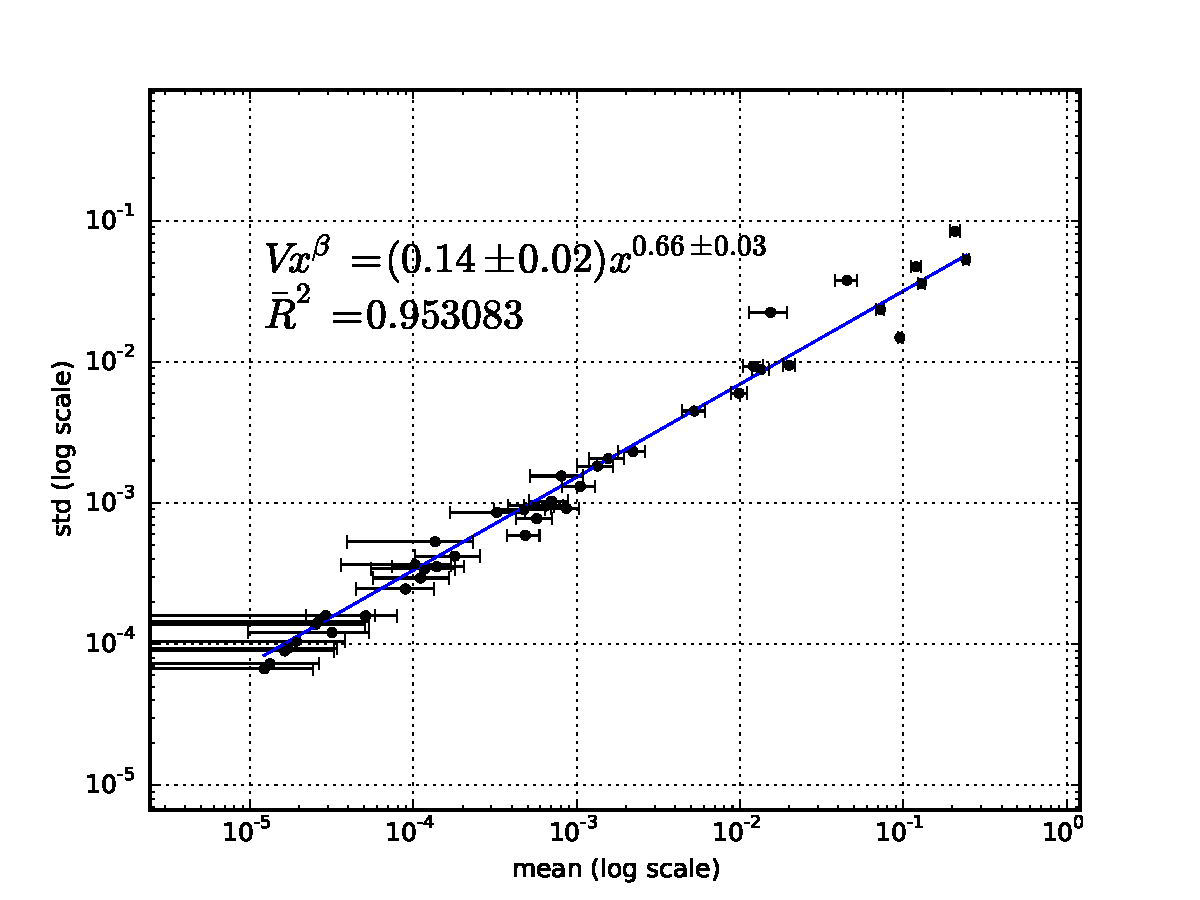
\includegraphics[width=0.8\textwidth]{results/fits/IBS_h_A_amplicons_family_stdVSmean_xWboot_LOG.pdf}
	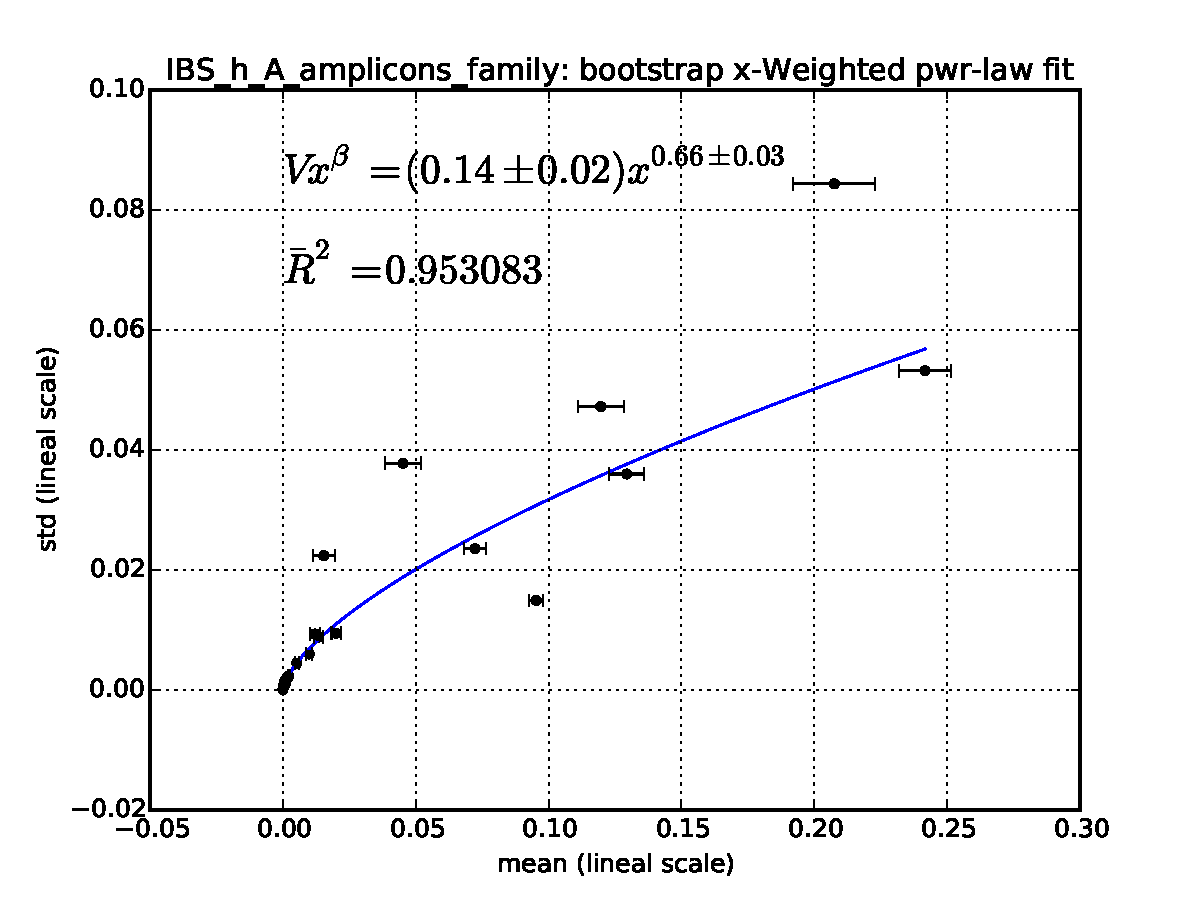
\includegraphics[width=0.8\textwidth]{results/fits/IBS_h_A_amplicons_family_stdVSmean_xWboot_LIN.pdf}
	\caption{The X-weighted fit log and lineal plots corresponding to the fit of Figure \ref{fig:unwFit}}
	\label{fig:X-wFit}
\end{figure}

\begin{figure}
	\centering
	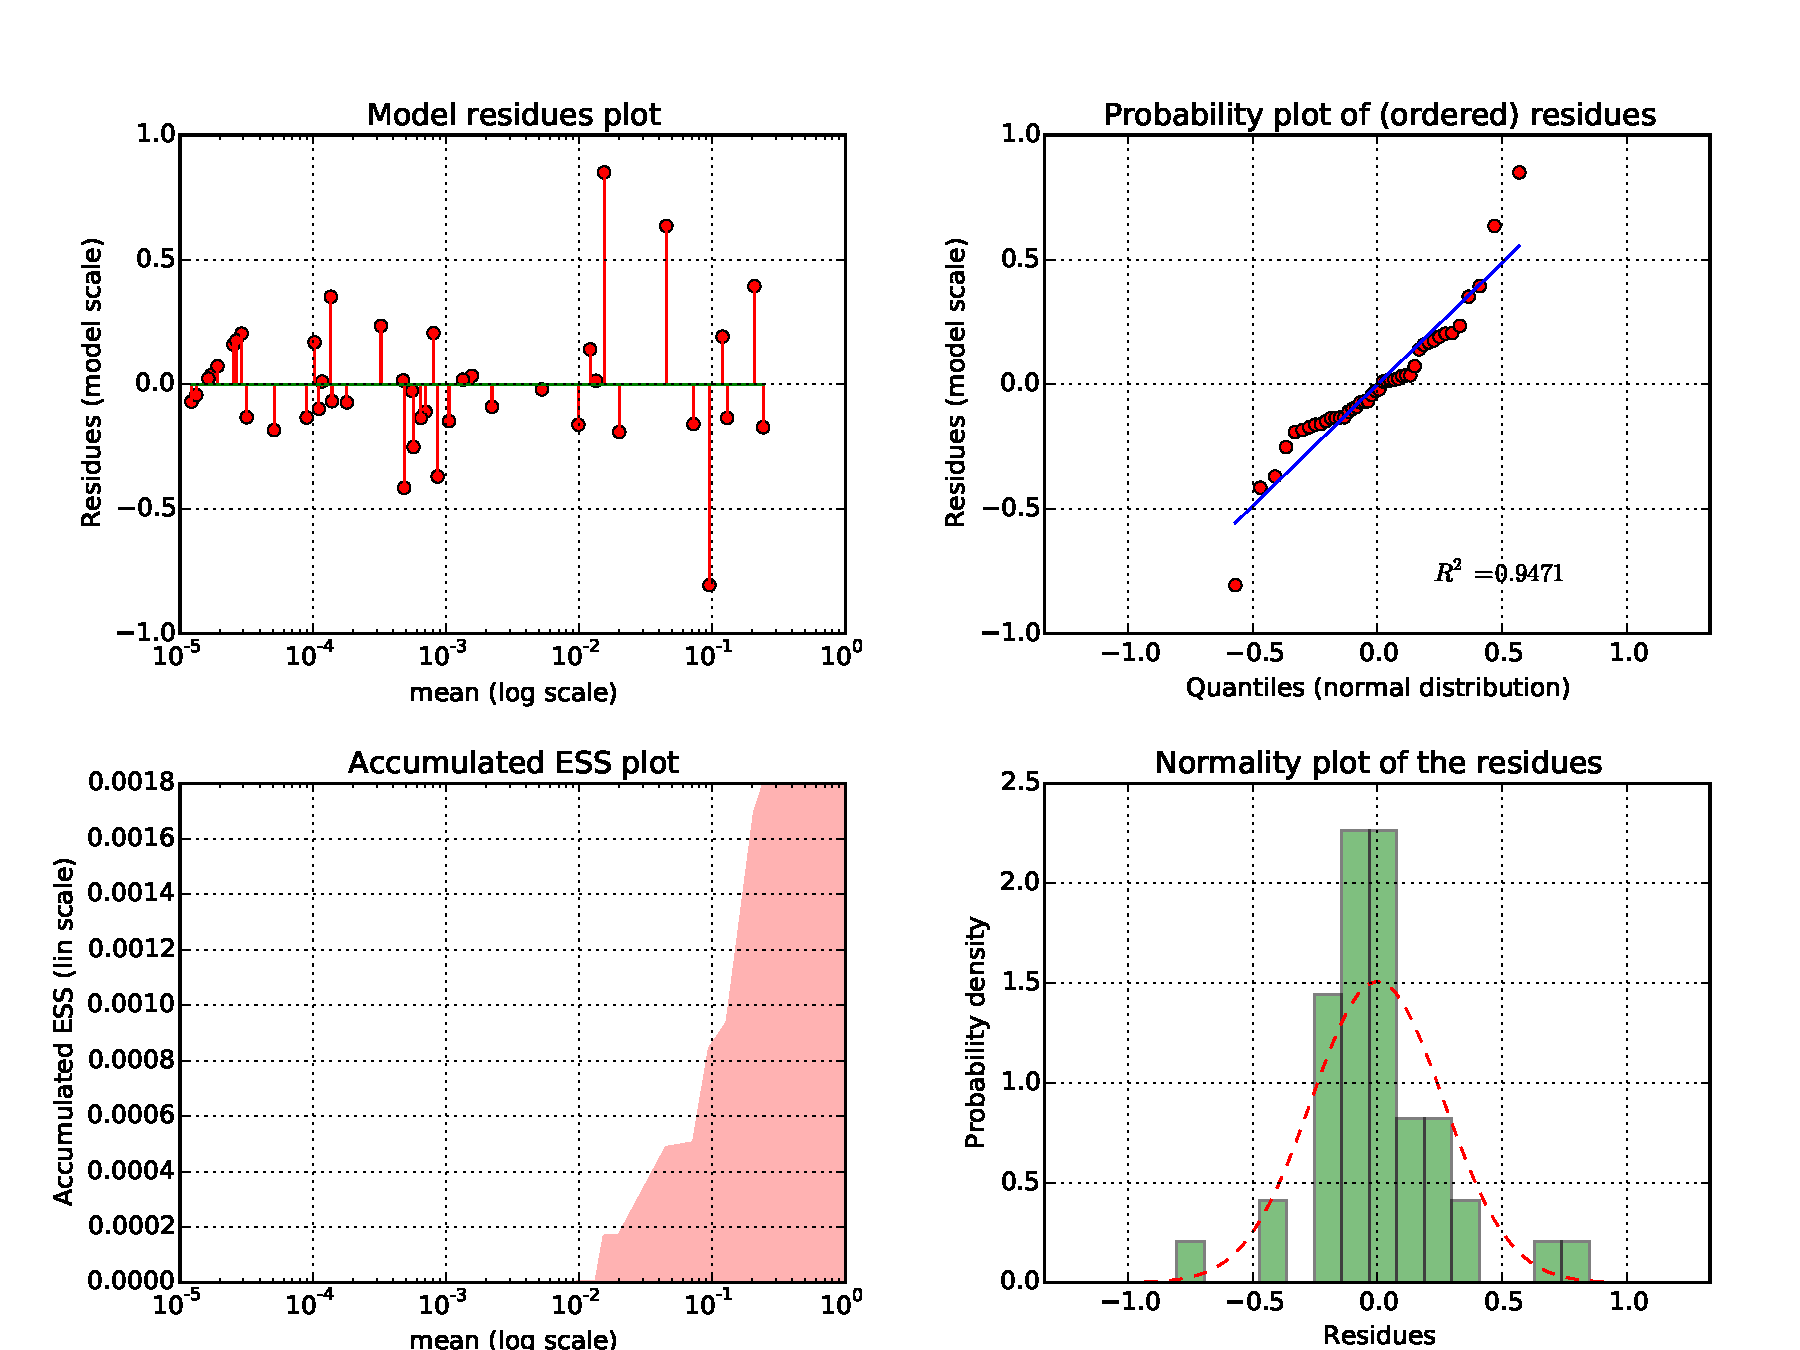
\includegraphics[width=\textwidth]{results/fits/IBS_h_A_amplicons_family_stdVSmean_LLR_RES.pdf}
	\caption{Residues analysis plot corresponding to the fit of Figure \ref{fig:unwFit}. The top-left subplot is a simple residues plot. The top-right subplot is a Normal quantiles plot with linear fitting (value of coefficient of determination is provided). The bottom-left subplot shows an accumulated ESS (Explained Sum of Squares) plot. Finally, the bottom-right subplot is a residues Normal histogram plot. This set of subplots allows to check for normality and homoscedasticity of the residues.}
	\label{fig:unwRes}
\end{figure}

\subsubsection*{Histogram Plots} 
\CC\ generates three different histogram plots:
\begin{description}
	\item[$-$Absolute frequencies plot]: This plot is useful to visually assess the validity of the time points in terms of the accumulated absolute frequency of the elements (taxa), since absolute frequencies far (much higher or much lower) from those typically observed could mean a sampling problem. As an example, Figure \ref{fig:histAFP} shows this histogram for the pre-treatment data (first 7 times) of patient ``D'' in the antibiotics study\cite{antibiotic}. 
	\item[$-$2D deviation plot]: The 2D semi-logarithmic histogram representing deviations from the mean versus the mean itself, is a useful tool in the analysis of the stability of ranking processes in complex systems\cite{ranking}. Figure \ref{fig:hist2D} shows this plot for the data used in the fit shown in Figure \ref{fig:unwFit}.
	\item[$-$Zero relative frequency plot]: We could define the ZRF (Zero Relative Frequency, thereby ranging from 0 to 1) of an element (taxon) as the portion of times where it is zero, i.e., it is not found. Attending to all the elements (taxa), we can plot the ZRF histogram, which then lies on the horizontal axis of the plot. The vertical axis shows the number of elements (taxa), so the height of a bar represents the number of elements that have determinate ZRF. In this respect, the bar over $0.0$ counts the number of elements (taxa) that are present at every time point of the data set (aka ``core''), while the bar over $1.0$ would count the number of elements (taxa) that are never found (this bar never appears because all these ``null'' elements are automatically filtered by the code). Figure \ref{fig:histZRF} shows an example of this plot. There, we can see that $12$ taxa are present at all the time points of the time series while $9$ taxa basically appear only once. So, this plot is clearly useful to notice how the ``core'' is distributed.
\end{description}

\begin{figure}
	\centering
	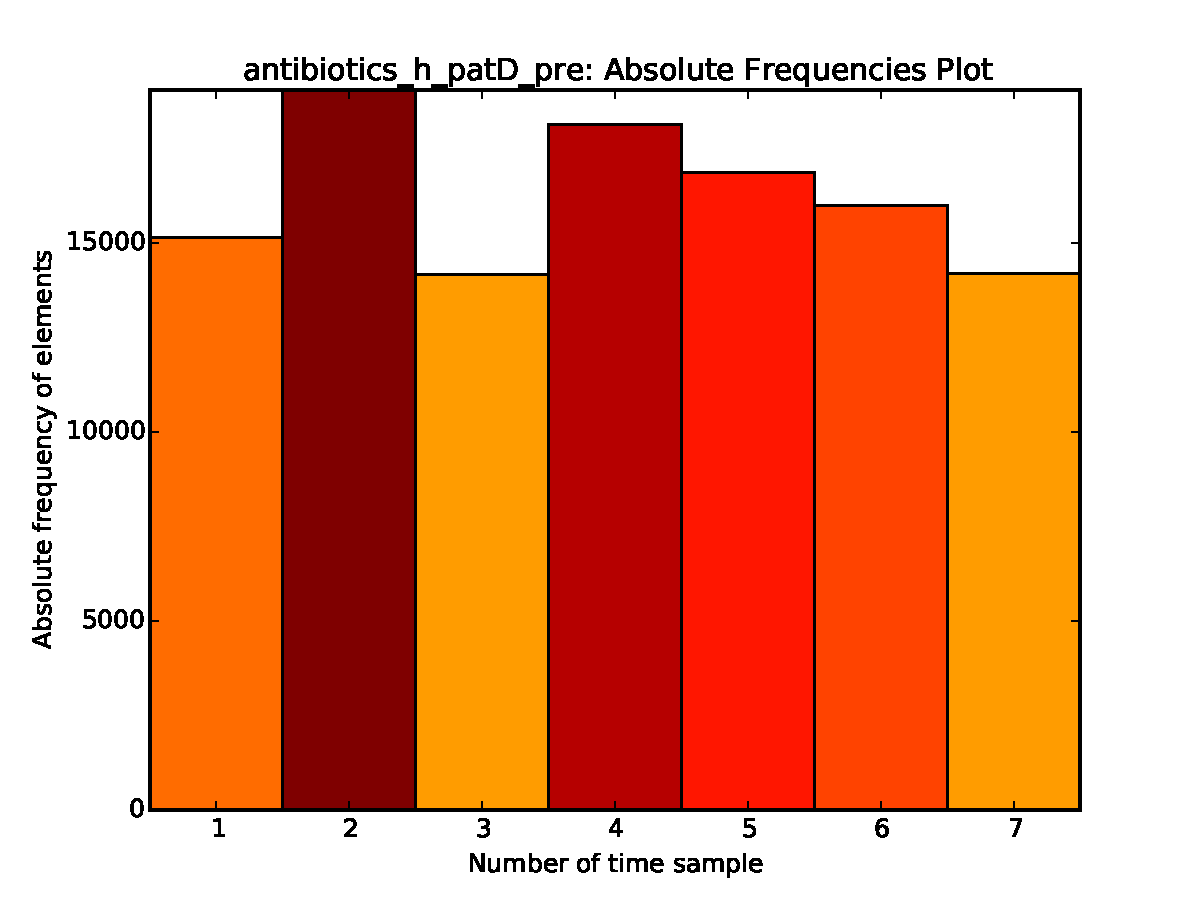
\includegraphics[width=0.8\textwidth]{results/hist/antibiotics_h_patD_pre_AbsFreqPlot}
	\caption{Histogram with the absolute frequencies of the pre-treatment data (7 first times) of patient ``D'' in the antibiotics study\cite{antibiotic}}
	\label{fig:histAFP}
\end{figure}

\begin{figure}
	\centering
	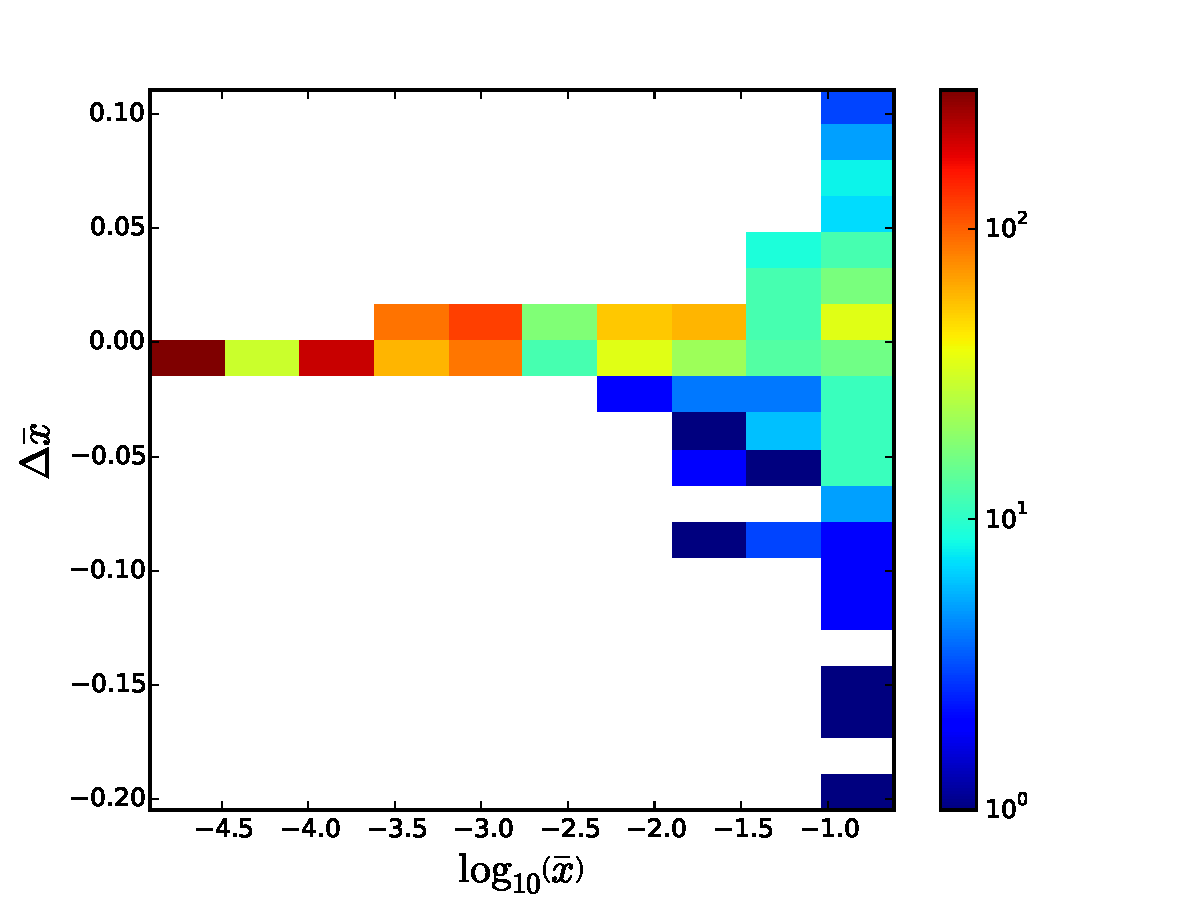
\includegraphics[width=0.8\textwidth]{results/hist/IBS_h_A_amplicons_family_hist2D.pdf}
	\caption{2D histogram deviation plot of the data used in the fit shown in Figure \ref{fig:unwFit}}
	\label{fig:hist2D}
\end{figure}

\begin{figure}
	\centering
	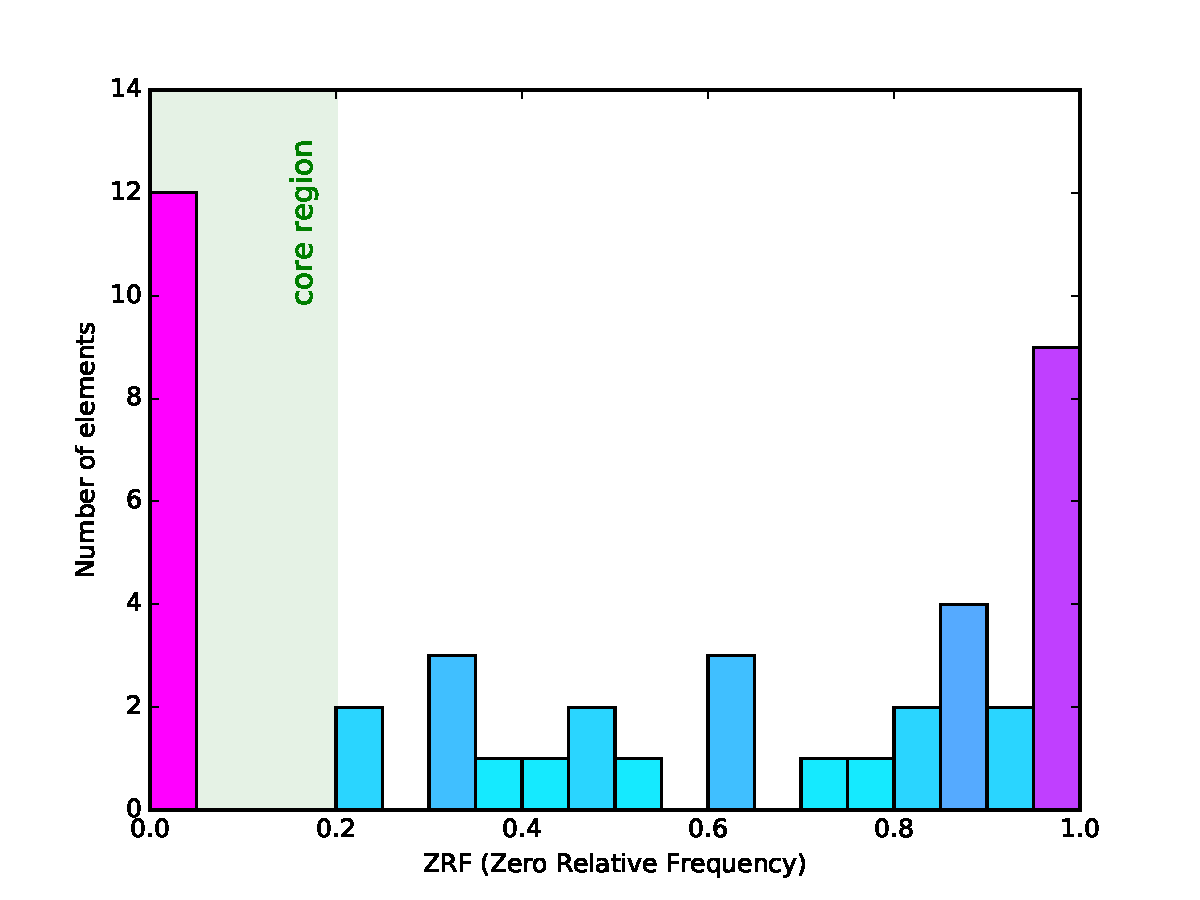
\includegraphics[width=0.8\textwidth]{results/hist/IBS_h_A_amplicons_family_ZRFhist.pdf}
	\caption{Histogram with the relative frequency of zero for the elements (taxa) in the data used in the fit shown in Figure \ref{fig:unwFit}}
	\label{fig:histZRF}
\end{figure}

\subsubsection*{Correlation and Rank Plots} 
\CC\ generates three different plots falling under this category, as well as Excel files with the resulting matrices:
\begin{description}
	\item[$-$Elements correlation matrix]: This plot shows a correlation matrix among the elements (taxa), calculated with the time as independent variable. For these calculations, the data set is not normalized to avoid entering an additional constraint. As an example, Figure \ref{fig:corrElm} shows this matrix for the ``core'' elements (taxa) present in the pre-treatment data (first seven times) of patient ``D'' in the antibiotics study\cite{antibiotic}. 
	\item[$-$Times correlation matrix]: This plot presents a correlation matrix among the time points of the data set, calculated with the elements (taxa) as independent variable. Again, the data set is not normalized. Figure \ref{fig:corrTim} shows this matrix for the ``core'' elements (taxa) present in pre-treatment data (first seven times) of patient ``D'' in the antibiotics study\cite{antibiotic}. 
	\item[$-$Rank dynamics and stability plot]: This plot shows the variation in the rank with time for the most dominant elements (taxa) and their calculated RSI, as discussed in Section \ref{sec:RSI}. Figure \ref{fig:corrank} shows this plot for the elements (taxa) in the data used in the fit shown in Figure \ref{fig:unwFit}.
\end{description}

\begin{figure}
	\centering
	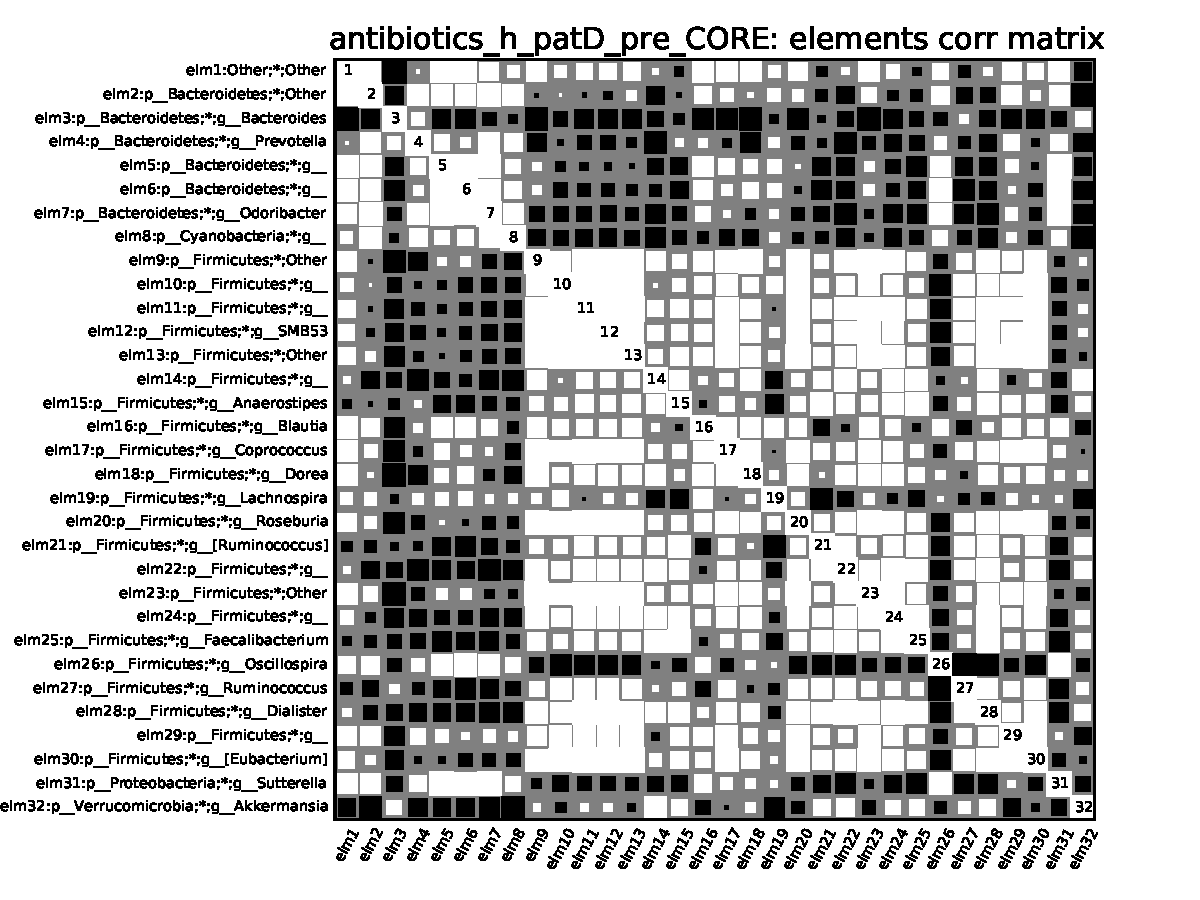
\includegraphics[width=0.9\textwidth]{results/corrank/antibiotics_h_patD_pre_CORE_ElementsCorr}
	\caption{Element correlation plot of the pre-treatment data (first seven times) of patient ``D'' in the antibiotics study\cite{antibiotic} for ``core'' taxa}
	\label{fig:corrElm}
\end{figure}

\begin{figure}
	\centering
	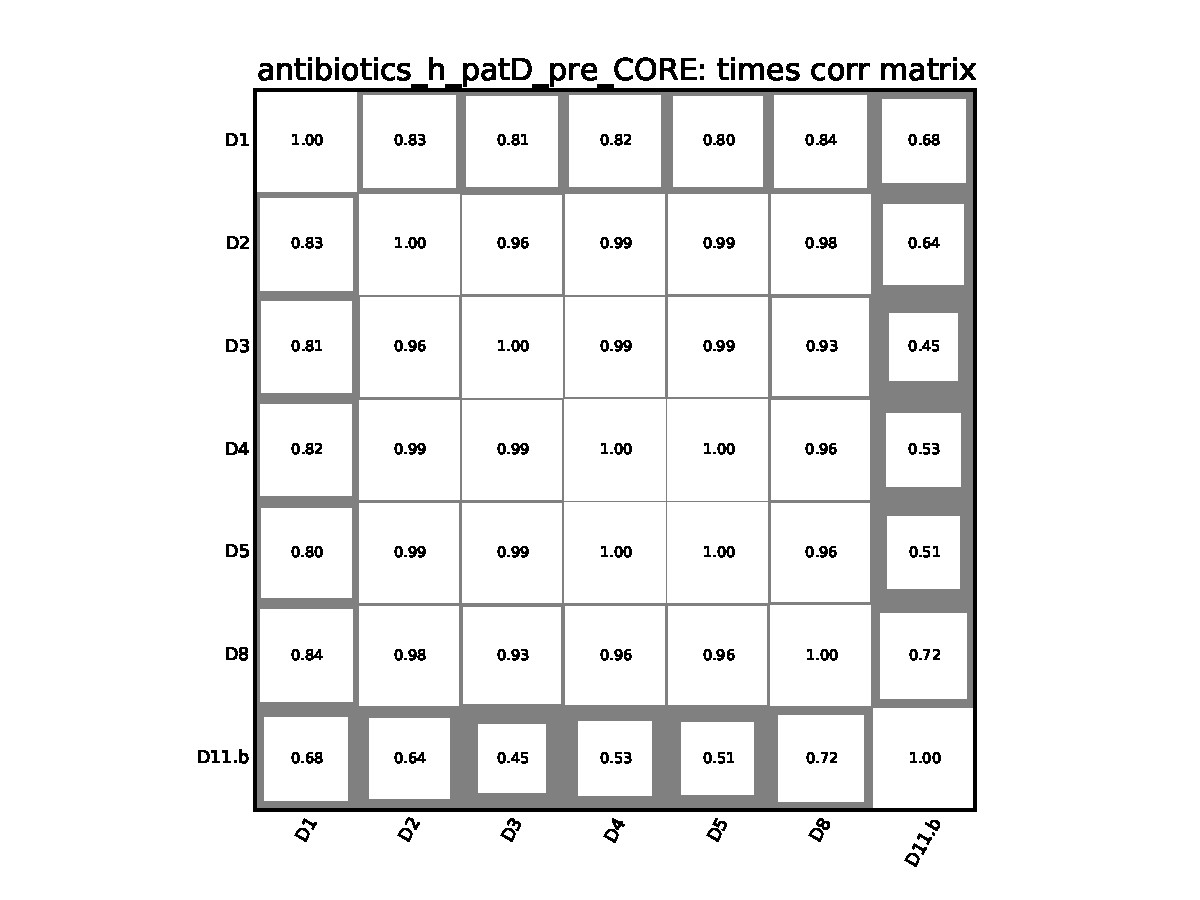
\includegraphics[width=0.9\textwidth]{results/corrank/antibiotics_h_patD_pre_CORE_TimesCorr}
	\caption{Times correlation plot of the pre-treatment data (first seven times) of patient ``D'' in the antibiotics study\cite{antibiotic} for ``core'' taxa}
	\label{fig:corrTim}
\end{figure}

\begin{figure}
	\centering
	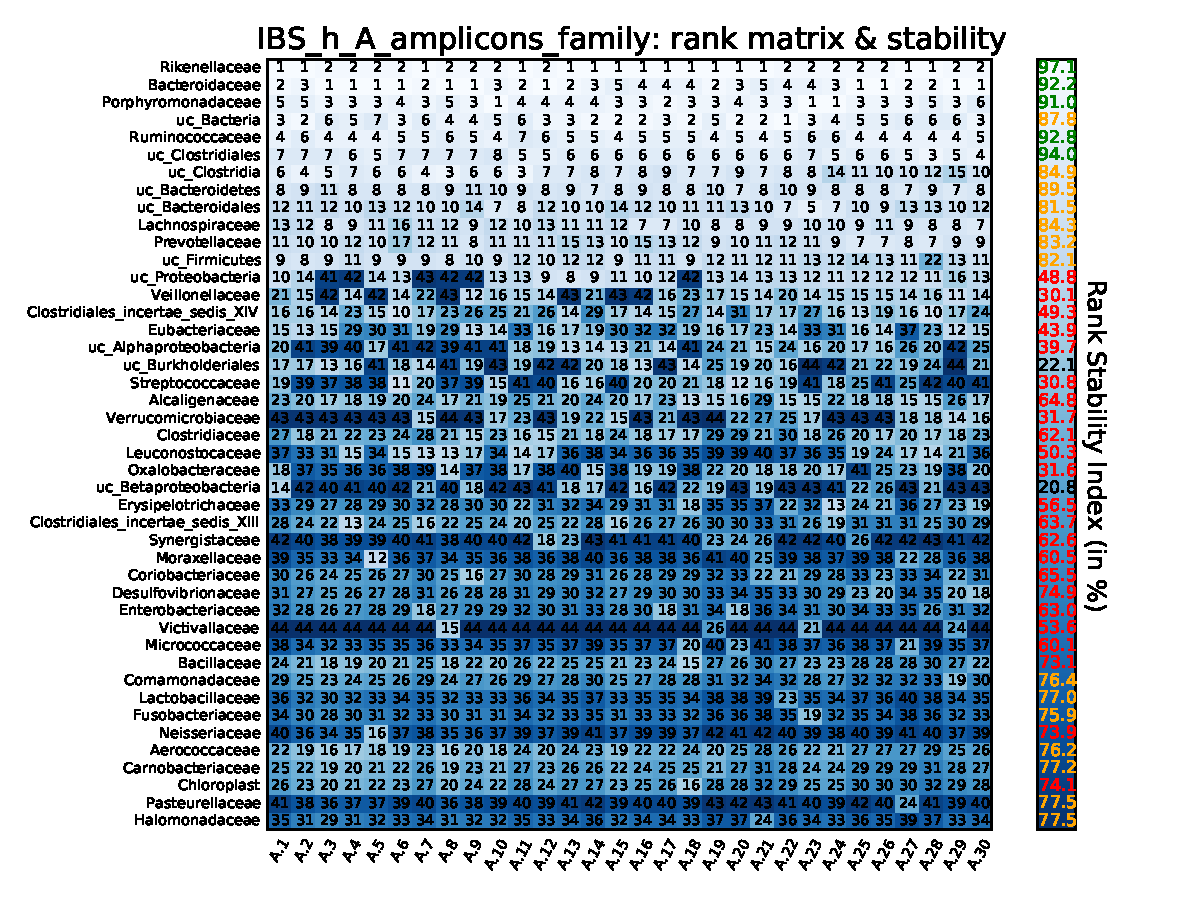
\includegraphics[width=\textwidth]{results/corrank/IBS_h_A_amplicons_family_Rank}
	\caption{Matrix showing the rank variation throughout time for the most dominant elements (taxa) and their calculated RSI (as discussed in Section \ref{sec:RSI}) in the data used in the fit shown in Figure \ref{fig:unwFit}}
	\label{fig:corrank}
\end{figure}

\subsection*{Standardization} \label{sec:stan}
In order to show all the studies properly under common axes, we decided to standardize the Taylor parameters using the group of healthy individuals for each study. With this approach, all the studies can be visualized in a shared plot with units of Taylor-parameters standard-deviation on their axes.

For a Taylor parameter, e.g. $V$, the estimate of the mean ($\widehat{V}$) for the healthy subpopulation, composed of $h$ individuals, is:
\begin{linenomath}
$$\widehat{V} = \frac{1}{W_1}\sum_{i=1}^h V_i \omega_i=\sum_{i=1}^h V_i \omega_i$$
\end{linenomath}
as $W_1=\sum_i^h \omega_i=1$, since $\omega_i$ are normalized weights calculated as:
\begin{linenomath}
$$\omega_i = \frac{\frac{1}{\sigma^2_{V_i}}}{\sum_i^h\frac{1}{\sigma^2_{V_i}}}$$
\end{linenomath}
being $\sigma_{V_i}$ the estimation of the uncertainty in $V_i$ obtained together with $V_i$ from the X-weighted power-law fit described in Section \ref{sec:X-w}, for healthy individuals.

Likewise, the estimation of the standard deviation for the healthy population ($\widehat{\sigma}_V$) is:
\begin{linenomath}
$$\widehat{\sigma}_V = \sqrt{\frac{1}{W_1-\frac{W_2}{W_1}}\sum_{i=1}^h\left[\omega_i\left(V_i-\hat{V}\right)^2\right]}$$
\end{linenomath}
being $W_2=\sum_i^h \omega_i^2$, which finally yields to:
\begin{linenomath}
$$\widehat{\sigma}_V = \sqrt{\frac{1}{1-\sum_i^h \omega_i^2}\sum_{i=1}^h\left[\omega_i\left(V_i-\hat{V}\right)^2\right]}$$
\end{linenomath}
